\documentclass[11pt]{article}
\usepackage[margin=1in]{geometry}
\usepackage[numbers,sort&compress]{natbib}
\usepackage{amsmath,amssymb}
\usepackage{booktabs}
\usepackage{graphicx}
\usepackage{tikz}
\usetikzlibrary{arrows.meta,positioning,calc}
\usepackage[hidelinks]{hyperref}
\usepackage{xcolor}
\usepackage{microtype}

\newcommand{\psilm}{$\Psi$LM}
\newcommand{\code}[1]{\texttt{#1}}
\newcommand{\pending}[1]{\textcolor{red!75!black}{\textbf{[pending: #1]}}}  % placeholder for numbers not yet in the committed logs

\title{\psilm: Coupling Frozen Language and Physics Models\\through Trainable Latent Bridges}

\author{Ryoji Furui\thanks{\url{https://github.com/ryoji-info/PsiLM}. \textbf{AI generation disclosure:} the research reported here was designed, implemented, executed, and written up by \emph{Claude} (Anthropic; the Claude Fable 5, Fable 5.1, and Opus 5 models, as recorded in the repository's commit trailers), working autonomously on the author's Apple M2 laptop under the author's direction; see Section~\ref{sec:disclosure}.}}
\date{September 11, 2026}

\begin{document}
\maketitle

\begin{abstract}
We ask whether a pretrained language model and a pretrained physics model can run as one system --- two frozen networks answering a single question with communication carried entirely by hidden states, the way the brain's hemispheres cooperate across the corpus callosum. As of August 2026 we find no published work coupling a pretrained LLM to a neural-operator physics model through a bidirectional latent channel at inference. We build such a system, \psilm{}, on a consumer laptop (Apple M2, 24\,GB), in five steps. (1) Tool-loop baselines reproduce the known capability-gap effect: a simulator adds $+28.3$ points to a 3B model on physics QA but \emph{hurts} a 0.5B model. (2) We produce, to our knowledge, the first public reproduction of the Bicameral Model \citep{flamant2026bicameral}: two frozen Qwen2.5-0.5B streams coupled by a 6.2M-parameter gated hidden-state interface reproduce the paper's phase transition, reaching 100\% exact tool recall through the latent channel alone. (3) With the auxiliary language model replaced by a frozen Fourier Neural Operator, \psilm{} answers Burgers-equation field-value questions at 100\% (tolerance $\pm 0.05$; MAE 0.014) where the LLM alone achieves 5\%, matching the accuracy of an oracle that states the answer in text --- with no text at the interface. (4) The result survives hardening: held-out question families expose a clean generalization law (\emph{support coverage} --- readouts generalize only where their training support covers the test distribution, a hypothesis we confirm by refuting the alternative), and the architecture transfers to 2D reaction--diffusion with a pretrained physics foundation model (DPOT-Tiny) as the hemisphere, scoring 95\%, within five points of the oracle ceiling. (5) The recipe then scales the language hemisphere to 1.7B, 8B, 12B and a mostly recurrent 9B backbone, where two families finish level with or above their text oracles (Gemma 4 12B: 96.7\% vs.\ 98.3\%; Qwen3.5 9B: 100\% vs.\ 98.3\%) with gates that stay shut off-task, GSM8K item-identical to the backbone. All experiments, including two failed designs and one refuted hypothesis, are reproducible from the public repository on a single consumer machine.
\end{abstract}

\section{Introduction}
\label{sec:intro}

Large language models reason in discrete tokens; physics foundation models \citep{barman2025lpm,hao2024dpot} evolve continuous fields. The human brain suggests a third architecture: specialized regions, neither subordinate to the other, co-processing a single task through dense internal communication. This paper takes the analogy literally. We couple a frozen pretrained LLM to a frozen pretrained physics model through small trainable \emph{bridges} operating purely on hidden states --- the language stream never sees the physics as text, and the physics model never parses a sentence --- and ask whether the coupled system can answer questions neither component can answer alone.

A second motivation is epistemic. In the wave--particle picture of quantum mechanics, a discrete observation is one reading of an underlying continuous process; Bohr called the two descriptions \emph{complementary}. \psilm{} instantiates that structure operationally: a continuous field evolved by a neural operator, and a discrete verbal reading of it produced by a language model, with a learned interface deciding what crosses between them. The name is the wave function $\Psi$.

Our literature survey (Section~\ref{sec:related}) found the ingredients of such a system published separately --- frozen-model latent bridges \citep{bansal2024calm,zolna2024gats}, two LLMs coupled in hidden-state lockstep \citep{flamant2026bicameral}, LLM--simulator loops through text \citep{liu2023mindseye,varambally2026zephyrus}, and brain-inspired shared workspaces \citep{vanrullen2021glw,goyal2022workspace} --- but no published coupling of a pretrained LLM to a neural-operator physics model through a bidirectional latent channel at inference, a gap independently noted as open by a survey of latent inter-model communication \citep{liu2026beyondtokens}. We fill it at small scale, on consumer hardware, with the following contributions:

\begin{enumerate}
\item \textbf{Baselines} (Sec.~\ref{sec:stage0}): a seeded physics-QA benchmark on which text-level tool coupling reproduces the published capability-gap effect ($+28.3$ points at 3B, $-3.3$ at 0.5B).
\item \textbf{A reproduction} (Sec.~\ref{sec:stage1}): the first public reimplementation of the Bicameral Model \citep{flamant2026bicameral}, confirming its training phase transition and its causal order, and documenting two facts the paper does not: an inference bootstrap required at the uncoupled prompt boundary, and a teacher-forced/rollout dissociation showing exposure bias dominates evaluation at this scale.
\item \textbf{\psilm{}} (Sec.~\ref{sec:psilm}): a frozen LLM and a frozen neural operator coupled through $\sim$3.5M trainable bridge parameters, reaching the oracle-text ceiling on 1D Burgers field-value QA (100\% vs.\ 5\% for the LLM alone).
\item \textbf{A generalization law} (Sec.~\ref{sec:gen}): on held-out question families the interface transfers partially, failure is attributable to a single readout, and a controlled experiment refutes the natural ``classify, don't regress'' fix --- establishing \emph{support coverage} as the operative principle.
\item \textbf{Foundation-model transfer} (Sec.~\ref{sec:2d}): the architecture carries to 2D reaction--diffusion with pretrained DPOT-Tiny \citep{hao2024dpot} as the physics hemisphere (95\% vs.\ 6.7\% alone).
\item \textbf{Scaling the language hemisphere} (Sec.~\ref{sec:scaling}): a backbone-agnostic parameterization and an MLX port carry the architecture to Qwen3-1.7B (93.3\% vs.\ a 96.7\% oracle) and to 4-bit backbones; a trained revision loop adds $+16.7$ points on the held-out combination family; and at Qwen3-8B a probe-by-probe analysis across eight runs locates two scale-dependent failures --- a learned attention pointer that never trains, and a field-carrying channel the frozen model shortcuts --- and the system that removes both closes to within a few points of its oracle; a guard-rail benchmark then shows its gate open on every prompt (a 55-point loss on GSM8K with the bridges attached), and a no-harm training arm makes the gate selective: GSM8K and MMLU return to the backbone's numbers with the physics result retained (Tables~\ref{tab:guardrail} and~\ref{tab:guardrail2}). The finished recipe then transfers in one pass to a second model family, Gemma 4 12B (96.7\% against a 98.3\% oracle, gate selective), with one measured, backbone-specific fix to the readout normalization (Sec.~\ref{sec:gemma}); and, in one further pass, to a third family whose decoder is mostly recurrent --- Qwen3.5 9B, 24 Gated DeltaNet (linear-attention) layers and 8 attention layers, NVFP4-quantized and rebuilt from an Ollama release --- where the readout warm-up ends, on twice the warm-up samples of the other backbones, at the best warm-up pointer in this work and the coupled system reaches 100\% on the held-out set against a 98.3\% oracle, with the gate selective --- GSM8K item-identical to the backbone (Sec.~\ref{sec:qwen35}).
\end{enumerate}

\section{Related Work}
\label{sec:related}

\textbf{Text- and tool-level coupling.} Mind's Eye \citep{liu2023mindseye} pioneered LLM reasoning grounded by a physics engine through prompt round-trips; RAP \citep{hao2023rap} framed reasoning as an agent conversing with a world model in text; Zephyrus \citep{varambally2026zephyrus} couples an LLM to numerical weather foundation models through code; SGA \citep{ma2024sga} alternates an LLM with differentiable simulation for scientific discovery; RIA \citep{sun2026ria} closes an LLM/world-model loop per decision step for driving. In all of these the physics side is a subroutine reached through text or code. Multiagent debate \citep{du2024debate} couples multiple reasoner instances through exchanged messages; Cicero \citep{bakhtin2022cicero} combines a language model with a strategic-reasoning module through structured intents. Position papers argue that language, agent, and world models must interoperate \citep{hu2023law,lecun2022ami}.

\textbf{Latent-level coupling.} Flamingo \citep{alayrac2022flamingo} and BLIP-2 \citep{li2023blip2} graft frozen perception onto frozen LLMs unidirectionally; CALM \citep{bansal2024calm} cross-attends between two frozen LLMs' layers; GATS \citep{zolna2024gats} exchanges activations bidirectionally among frozen models at different rates. Socratic Models \citep{zeng2023socratic} made language itself the inter-model protocol; a fast-moving line replaces it with embeddings, activations, or KV state \citep{pham2024cipher,ramesh2025activations,zou2025latentmas,liu2026wormhole,shen2024collm,rodionov2025hogwild,wang2025parallelsurvey}; DroidSpeak \citep{liu2024droidspeak} shows even same-architecture models need repair to share raw state, motivating trained interfaces. Closest to our Stage~1, the Bicameral Model \citep{flamant2026bicameral} runs two frozen LLMs in per-token lockstep through a trainable gated interface; no code was released.

\textbf{Brain-inspired modular systems.} The Global Workspace line \citep{vanrullen2021glw,devillers2023gw,maytie2025gwdreamer,goyal2022workspace} couples frozen specialists through a learned shared latent space; bilateral architectures \citep{rajagopalan2022bilateral,rinaldo2024leftright} build literal two-hemisphere networks with an ablated callosal channel; \citet{bena2024specialization} show module specialization requires a bandwidth-constrained channel. Dual-process agents \citep{booch2021sofai,deepmind2024talker} and dual-system robot policies \citep{figure2025helix,nvidia2025groot} run a slow semantic model and a fast control model concurrently over latent interfaces.

\textbf{Language and PDE operators.} UPS \citep{shen2024ups} projects FNO features into a pretrained LLM's token space; Unisolver \citep{zhou2025unisolver} conditions a neural solver on frozen-LLM equation embeddings; ICON-LM \citep{yang2025iconlm} fine-tunes a GPT-2 into an operator learner; Text2PDE \citep{zhou2025text2pde} generates rollouts from text; \citet{negrini2025multimodalpde} decode operator states into text within one purpose-trained network. Each realizes one direction, or fuses everything into a single network; none couples two \emph{pretrained} models bidirectionally at inference.

\section{Experimental Platform}
All experiments run on one Apple M2 laptop with 24\,GB unified memory. The language hemisphere is frozen Qwen2.5-0.5B-Instruct \citep{qwen2025qwen25} (hereafter Qwen2.5-0.5B; fp16 on PyTorch MPS; 4-bit MLX quantizations for Stage~0; Section~\ref{sec:scaling} substitutes larger Qwen3, Gemma 4, and Qwen3.5 backbones), staged so a forward pass can pause at any decoder layer, exchange state, and resume; the staged pass is bit-exact against the stock model. Ground truth for the PDE tasks (Sections~\ref{sec:psilm}--\ref{sec:2d}) comes from spectral solvers with integrating-factor RK4 (dt-convergence $\le 4\times10^{-11}$; analytic limits verified), never from the neural physics models; Stages 0--1 are scored against closed-form mechanics and exact arithmetic. Trained components are only the interfaces (2--7M parameters on the 0.5B backbone; 12.6M for the 1.7B and 40--45M for the larger backbones of Section~\ref{sec:scaling}); training runs in resumable 500--1000-step chunks at 1.8--12\,s/step depending on the backbone.

\section{Stage 0: Text-Level Tool Coupling}
\label{sec:stage0}
We construct a seeded 60-item benchmark of rigid-body comparison questions (five scene types; one third are physics traps such as equal-mass free fall and complementary launch angles) scored against closed-form mechanics, and evaluate an \emph{alone} arm against a \emph{tool} arm in which the LLM extracts scene parameters as JSON, a simulator computes the outcome, and the result returns to the prompt \citep{liu2023mindseye}. Parameter extraction succeeds on 100\% of items at both model sizes, yet coupling helps only the larger model: Qwen2.5-3B improves $38.3\%\!\to\!66.7\%$ ($+28.3$, matching Mind's Eye's published $+27.9$ zero-shot average), while Qwen2.5-0.5B \emph{degrades} $35.0\%\!\to\!31.7\%$ --- it cannot reliably compare two numbers handed to it in text. Evidence \emph{use}, not extraction, is the bottleneck, motivating a trained interface that delivers evidence below the token level.

\section{Stage 1: Reproducing the Bicameral Model}
\label{sec:stage1}

We reimplement the Bicameral Model \citep{flamant2026bicameral} from its published specification: two frozen Qwen2.5-0.5B streams generate in lockstep; a trainable interface reads the primary's residual stream at layer 10 and writes a gated update into the auxiliary at layer 10 (forward coupling), and symmetrically auxiliary$\to$primary at layer 15 (reverse), each update $h \leftarrow (1-\sigma)h + \sigma f(h_{\text{send}})$ with the suppression gate $\sigma$ computed from the \emph{receiver}. The auxiliary drives a calculator whose output is forced into the auxiliary stream only; the primary receives results exclusively through the latent channel. We train the 6.2M-parameter interface with dual-target SFT on procedurally generated multiplication problems carrying causality-aligned auxiliary traces (192k samples).

\begin{figure}[t]
\centering
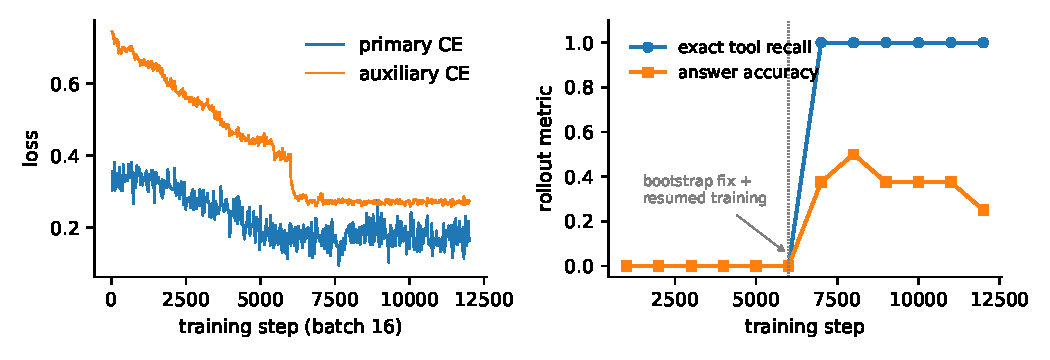
\includegraphics[width=\linewidth]{figs/stage1.pdf}
\caption{Stage 1 reproduction. \textbf{Left:} teacher-forced losses. \textbf{Right:} rollout metrics per 1000-step chunk. Exact tool recall undergoes the paper's phase transition ($0\!\to\!1.00$ within one chunk, at $\sim$112k samples) after an inference-bootstrap fix at step 6000; answer accuracy sets in after recall, in the paper's causal order.}
\label{fig:stage1}
\end{figure}

\textbf{The phase transition reproduces, in its causal order} (Fig.~\ref{fig:stage1}): forward coupling strengthens first, exact tool recall then jumps $0.00\!\to\!1.00$ in a single chunk, and answer accuracy sets in afterward. On held-out problems (7--10-digit products) the coupled system emits the exact \code{calc(A*B)} on 100\% of rollouts --- the auxiliary reads the operands entirely from hidden states --- while the reverse channel carries the leading 4--6 result digits reliably and degrades toward the tail (digit similarity 0.689 vs.\ 0.371 for the frozen model alone; exact match only 2.5\% at this length, $\sim$25--50\% on the shorter mixed-length products of the per-chunk rollout evaluations, $n{=}8$ each).

Two findings absent from the original paper: (i) the first auxiliary token is predicted from the \emph{uncoupled} prompt tail, a position training can never influence, so free-running generation derails without a protocol-level bootstrap (we force two initial wait tokens); (ii) high teacher-forced channel quality coexists with zero rollout success until that bootstrap exists --- exposure bias dominates evaluation at this scale (the committed diagnostic at the final checkpoint, \code{teacher\_forced\_diagnostic.json}: 100\% call-token accuracy and 63.0\% per-digit accuracy, against 0\% rollouts before the bootstrap).

\section{\psilm{}: A Language Model Coupled to a Neural Operator}
\label{sec:psilm}

\begin{figure}[t]
\centering
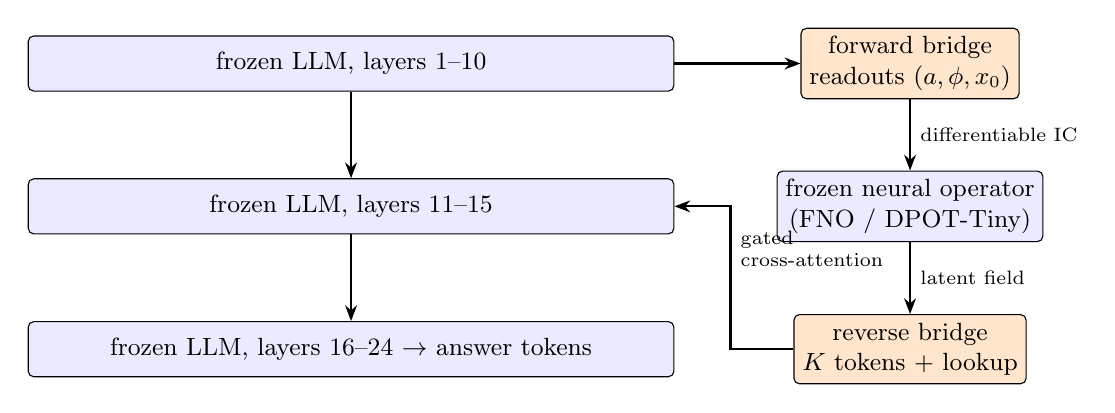
\begin{tikzpicture}[font=\small, node distance=4mm,
  box/.style={draw, rounded corners=2pt, minimum height=7mm, inner sep=3pt},
  frozen/.style={box, fill=blue!8},
  train/.style={box, fill=orange!20},
  arr/.style={-{Stealth[length=2mm]}, thick}]
\node[frozen, minimum width=82mm] (l10) {frozen LLM, layers 1--10};
\node[frozen, minimum width=82mm, below=11mm of l10] (l15) {frozen LLM, layers 11--15};
\node[frozen, minimum width=82mm, below=11mm of l15] (l24) {frozen LLM, layers 16--24 $\rightarrow$ answer tokens};
\node[train, right=16mm of l10.east, align=center, anchor=west] (fwd) {forward bridge\\readouts $(a,\phi,x_0)$};
\node[frozen, align=center] (fno) at (fwd |- l15) {frozen neural operator\\(FNO / DPOT-Tiny)};
\node[train, align=center] (rev) at (fwd |- l24) {reverse bridge\\$K$ tokens + lookup};
\draw[arr] (l10.east) -- (fwd.west);
\draw[arr] (fwd) -- (fno) node[midway, right, font=\scriptsize]{differentiable IC};
\draw[arr] (fno) -- (rev) node[midway, right, font=\scriptsize]{latent field};
\draw[arr] (rev.west) -- ++(-8mm,0) |- (l15.east) node[pos=0.35, right, font=\scriptsize, align=left]{gated\\cross-attention};
\draw[arr] (l10) -- (l15);
\draw[arr] (l15) -- (l24);
\end{tikzpicture}
\caption{\psilm{}. Orange components (3.5--3.7M parameters) are the only trained ones. The question is read out of the LLM's layer-10 hidden states; the frozen operator evolves the field; the result returns through a position-lookup token and gated cross-attention at layer 15. No text crosses the interface.}
\label{fig:arch}
\end{figure}

Stage 2 replaces the auxiliary language model with a genuine physics model (Fig.~\ref{fig:arch}). The task: ``$u(x,0)=a\sin(2\pi x+\phi)$ evolves by Burgers' equation ($\nu=0.02$) until $t=0.5$; what is $u$ at $x_0$?'' --- answered to two decimals, scored within $\pm 0.05$ on fields spanning $\pm 0.6$ (a degenerate always-zero strategy scores 7.9\% on the training distribution and 1.7\% on the held-out set of Table~\ref{tab:main}). The physics hemisphere is a 70k-parameter FNO trained once on solver data to $0.28\%$ relative error (one-shot $u_0 \mapsto u(\cdot,T)$, in the full-rollout style of contemporary physics foundation models) and then frozen.

\textbf{Forward bridge (language$\to$physics).} Learned queries attention-pool the LLM's layer-10 prompt states; heads regress $(a,\sin\phi,\cos\phi)$ and read the query position $x_0$ as a 100-way classification whose softmax expectation is differentiable and sharp. A differentiable sinusoid built from the readout feeds the operator, so answer-loss gradients flow from the LLM's words into the physics input.

\textbf{Reverse bridge (physics$\to$language).} $K{=}16$ learned queries compress the operator's latent field (plus Fourier positional features and the predicted field itself) into soft tokens, joined by a \emph{position-lookup token}: a periodic von Mises kernel of learnable sharpness, centered at the $x_0$ readout, samples the field ``where the question asked,'' with an auxiliary head deep-supervised on $u(x_0)$. All tokens enter the primary at layer 15 through gated cross-attention (receiver-computed suppression gate, near-closed initialization).

\textbf{Training} minimizes answer cross-entropy plus auxiliary readout losses (parameter MSE, $x_0$ CE, lookup-value MSE); both backbone networks stay frozen. Two design elements were forced by failure analysis, which we report as results. Plain cross-attention over field summaries mode-collapsed to per-trajectory constants (the system answered the field's \emph{average} for every $x_0$), and a regressed $x_0$ (RMS error 0.06) was too blurry beside a shock; the classification pointer and the deep-supervised lookup cracked both. First-chunk rollout accuracy was 0.08 for both failed designs, then 0.50 and 1.00 in the final design's first two 16k-sample chunks (Fig.~\ref{fig:chunks}, left, shows all three configurations).

\begin{table}[t]
\centering
\caption{Held-out results. Left: 1D Burgers ($n{=}60$). Right: 2D Fisher--KPP with pretrained DPOT-Tiny ($n{=}60$). Tolerance $\pm0.05$; greedy decoding; all arms share the frozen Qwen2.5-0.5B.}
\label{tab:main}
\small
\begin{tabular}{lrr@{\hspace{8mm}}rr}
\toprule
 & \multicolumn{2}{c}{1D Burgers (FNO)} & \multicolumn{2}{c}{2D Fisher--KPP (DPOT-Tiny)} \\
arm & acc@0.05 & MAE & acc@0.05 & MAE \\
\midrule
LLM alone & 5.0\% & 0.729 & 6.7\% & 0.337 \\
LLM + answer in text (oracle) & 100\% & 0.0028 & 100\% & 0.0024 \\
\textbf{\psilm{} (latent coupling)} & \textbf{100\%} & \textbf{0.0138} & \textbf{95.0\%} & \textbf{0.0168} \\
degenerate always-0.00 & 1.7\% & 0.308 & 1.7\% & 0.673 \\
\bottomrule
\end{tabular}
\end{table}

\textbf{Result} (Table~\ref{tab:main}, left): \psilm{} answers 100\% of held-out questions within tolerance (MAE 0.0138), matching the accuracy of an oracle that states the true value in the prompt --- while the frozen LLM alone scores 5\%. The answer travels entirely through hidden states: question out of the residual stream, simulation in the operator, value back through gated attention, verbalized by a frozen model.

\begin{figure}[t]
\centering
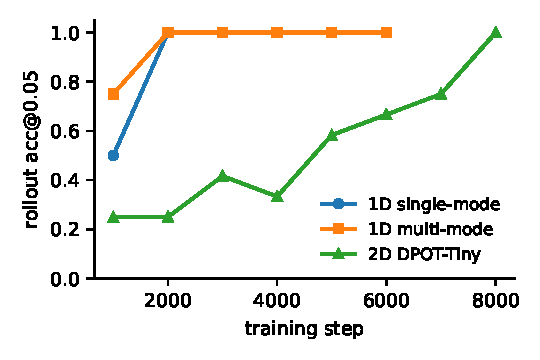
\includegraphics[width=0.48\linewidth]{figs/stage2_chunks.pdf}\hfill
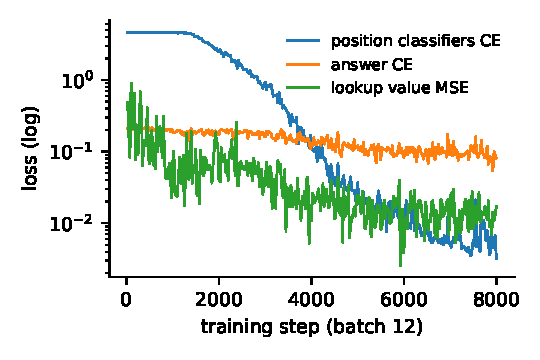
\includegraphics[width=0.48\linewidth]{figs/stage2d_phases.pdf}
\caption{\textbf{Left:} rollout accuracy per training chunk for the three \psilm{} configurations. \textbf{Right:} 2D training phase structure --- the four positional classifiers lock in first (over $\sim$5k steps); the answer loss converges only after the pointer does, echoing Stage~1's causal ordering.}
\label{fig:chunks}
\end{figure}

\section{Generalization: the Support-Coverage Law}
\label{sec:gen}

To harden the result we extend the initial conditions (ICs) to sums of sinusoids and train the bridges \emph{only on single-mode questions}, evaluating on three families: in-distribution, the held-out combination (two-term questions never seen), and amplitude extrapolation beyond the training range. The physics FNO is trained on a broader distribution than any evaluation family, so transfer failures are attributable to the interface. Results ($n{=}48$ per family): in-distribution 97.9\% (MAE 0.009); unseen combination 31.3\% (0.128); extrapolation 50.0\% (0.096) --- all above the LLM-alone (0--6.3\%) and always-zero (27.1\%, 16.7\%, 4.2\%) baselines, decisively so except against the combination family's zero baseline, and both transfer families far below in-distribution.

Teacher-forced attribution is unambiguous: the $x_0$ pointer generalizes \emph{perfectly} to every family (absolute error $\le 10^{-4}$), while the amplitude readout alone degrades $0.043 \to 0.355$ (combination) and $0.206$ (extrapolation); the record is committed as \code{attribution.json}. The natural hypothesis --- the classified quantity transfers, so classify the amplitudes too --- we tested with a v2 interface (per-mode pooling queries; amplitudes as 121-bin classifications). \textbf{It was worse on every family} (in-distribution $98\%\!\to\!94\%$, extrapolation $50\%\!\to\!19\%$, combination $31\%\!\to\!21\%$; v2 was evaluated at its 64k-sample convergence plateau --- rollout accuracy flat across its final two chunks --- vs.\ v1's 96k). The refutation identifies the real principle: $x_0$ generalized because all 100 of its bins occur in training, whereas amplitude bins outside the trained range never receive gradient and cannot move, while regression at least drifts. We summarize this as a \emph{support-coverage law}: a trained latent interface generalizes like a learned model, not a program --- coverage of the readout's support at training time, not the readout's parameterization, is what buys transfer. Section~\ref{sec:gemma-multimode} sharpens it at 12B into two coverages that can be bought separately --- structure and value --- and reports which of the two the refuted v2 interface was missing. Section~\ref{sec:2d} applies the law prospectively.

\section{2D Physics with a Pretrained Foundation Model}
\label{sec:2d}

Finally, we replace our own operator with DPOT-Tiny \citep{hao2024dpot}: a 7.5M-parameter AFNO operator pretrained across twelve PDE datasets, loaded with \code{strict=True} from the published checkpoint, fine-tuned for 1200 steps ($\approx$5 minutes) to 1.64\% relative error on our task, then frozen. The task moves to 2D Fisher--KPP reaction--diffusion on the periodic unit square: a Gaussian bump --- height, center, and width all stated in the question --- grows and spreads by $u_t = D\nabla^2 u + r\,u(1-u)$, and the question asks for $u$ at a point $(x_0,y_0)$ sampled within the front's active zone (always-zero scores 4.8\% on the training distribution; 1.7\% held-out). The IC is replicated across DPOT's 10-timestep input history; the reverse bridge attends over DPOT's 256 latent patch tokens plus a separable 2D periodic lookup on the predicted field; applying the support-coverage law, we make every positional readout (bump center and query point) a fully covered 100-bin classification.

Training exhibits a clean phase structure (Fig.~\ref{fig:chunks}, right): the four positional classifiers lock in over $\sim$5k steps (CE $4.6\!\to\!0.04$), and the answer loss converges only after the 2D pointer does; rollout accuracy climbs $0.25 \to 1.00$ over 96k samples. Held-out (Table~\ref{tab:main}, right): \textbf{95.0\%} at MAE 0.0168, within five points of the oracle-text ceiling, against 6.7\% for the LLM alone. The 1D result survives both moves --- to 2D, and to a physics hemisphere that is a genuine pretrained foundation model.

\textbf{The same task at 12B.} Rerunning Stage 2d on Gemma 4 12B (the recipe of Section~\ref{sec:gemma}, 7,500 steps: 2,000 readout-only, 4,000 coupled, 1,500 no-harm; \code{results/stage2d\_gemma12b\_2d/}) gives \textbf{100\%} at MAE 0.0096 on sixty held-out questions, against 10.0\% for the backbone alone and \textbf{96.7\% for the oracle} --- the first arm in this work where the latent channel beats the text ceiling (Qwen3.5 repeats it on the 1D task, Section~\ref{sec:qwen35}). The mechanism is mechanical rather than mysterious: the oracle must copy a number out of the prompt and occasionally mis-rounds it (MAE 0.021), while the bridge reads the field value exactly and the answer never passes through text (0.0096). The coupled phase ended at 93.8\% and the no-harm phase ran 97.9\%, 95.8\%, 100\%, so gate selectivity again cost nothing on the task. One engineering note for hybrid stacks: MLX and PyTorch share one unified GPU memory and MLX's cached buffers are invisible to PyTorch's MPS allocator, so the no-harm arm --- whose prompts are the long ones --- died asking for 256 bytes with 42\,GiB in ``other allocations''; returning the cache at the boundary was not sufficient and the physics model (7.5M parameters) simply runs on the CPU, at 65\,ms against 48\,ms per batch-4 call.

\section{Scaling the Language Hemisphere}
\label{sec:scaling}

Stage~0 predicts that the payoff of coupling grows with the language model's ability to \emph{use} evidence. This section reports what happened when the language hemisphere was scaled from 0.5B to 1.7B, 8B, 9B and 12B parameters with the physics hemisphere (the Stage-2 FNO, byte-identical) and the task held fixed. The 1.7B result is a clean transfer. The 8B was not, and we report it as a scale-dependent failure analysis in the spirit of Sections~\ref{sec:psilm} and~\ref{sec:gen}: each step isolates one component, and the sequence ends in a decision, a concession, a system that works on its task for a reason we can state, a guard-rail measurement of what it cost off-task, and the training arm that removed the cost. The finished recipe is then carried to two further families, Gemma 4 12B (Section~\ref{sec:gemma}) and the mostly recurrent Qwen3.5 9B (Section~\ref{sec:qwen35}); between them, the multi-mode task is rerun at 12B (Section~\ref{sec:gemma-multimode}) and an inference-time sweep (Section~\ref{sec:leaky}) bounds what an always-on channel costs.

\subsection{Backbone parameterization and Qwen3-1.7B}
\label{sec:scaling17}

The interface is parameterized by the backbone's configuration alone: coupling depths are the Stage-2 fractions of depth (read at $10/24$, inject at $15/24$, rounded; Qwen3.5 alone injects deeper, at $26/32$, for the memory reason given in Section~\ref{sec:qwen35}), bridge widths follow the hidden size, and the staged forward pass is verified bit-exact against the stock model for every new backbone before training. On Qwen3-1.7B \citep{qwen2025qwen3} (28 layers, hidden 2048; fp16 on PyTorch MPS; thinking mode disabled) the bridges resize to 12.6M parameters, couple at layers 12/18, and train at 5.2\,s/step. Under the Stage-2 budget (5000 steps $\times$ 16 = 80k samples) the per-chunk rollout probe reaches 1.00 in the fifth chunk, and the held-out evaluation ($n{=}60$, the set of Table~\ref{tab:main}) gives \textbf{93.3\%} at MAE 0.022 against an oracle-text ceiling of 96.7\% (MAE 0.021), with the LLM alone at 1.7\% (MAE 2.57) and the always-zero strategy at 1.7\%. Two observations. First, the receiver-computed gate, which settles at $\sigma\approx0.13$ on the 0.5B, opens fully ($\sigma\to1.0$) within the first 25 steps on the 1.7B and stays there: the stronger backbone takes the channel at full strength. Second, an evaluation-protocol lesson: the terse ``reply with only the number'' instruction that worked at 0.5B made Qwen3-1.7B's non-thinking mode drop minus signs systematically (oracle 47\%, half the negatives wrong, while free-form answers were correct). All text arms now use an ``\code{Answer:\ <number>}'' marker with marker-aware parsing, under which the coupled and oracle arms of Table~\ref{tab:main} reproduce (100\%/0.0138 and 100\%).

\subsection{Loop coupling: revision buys composition}
\label{sec:loop}

Before scaling the backbone we asked whether the interface itself had headroom on the Section~\ref{sec:gen} families. \code{loop\_model.py} runs two read$\to$rollout$\to$inject passes ordered $r_1<w_1<r_2<w_2$ (layers 8/11, then 15/18 of 24), so the second readout sees the stream \emph{after} the first injection and can revise it; the bridges are shared across passes (a recurrence), every pass's readouts are supervised, and the answer loss is applied once. Table~\ref{tab:loop} compares it with the single-pass interface at a matched 96k-sample budget, plus a third arm that simply runs the single-pass-trained bridges as two passes at inference. \textbf{The trained loop buys compositional generalization}: $+16.7$ points on the unseen combination family, with MAE improved on every family (the extrapolation error nearly halves at flat accuracy --- support coverage still rules there). The third arm collapses: switching the loop on at run time without training it is catastrophic, not neutral, with the caveat that this arm changes the coupling depths and the untrained revision at once, so it bounds the zero-shot transplant rather than isolating the revision effect. Loops must be trained in; they then pay off exactly where the single-pass interface was weakest.

\begin{table}[t]
\centering
\caption{Loop-coupling ablation on the multi-mode task of Section~\ref{sec:gen} (\psilm{} arm; $n{=}48$ per family; acc@0.05 / MAE; both trained arms at 96k samples).}
\label{tab:loop}
\small
\begin{tabular}{lrrr}
\toprule
family & single pass & loop-trained & inference-only loop \\
\midrule
in-distribution & 97.9\% / 0.009 & \textbf{100\%} / 0.007 & 8.3\% / 0.323 \\
unseen combination & 31.3\% / 0.128 & \textbf{47.9\%} / 0.089 & 0.0\% / 0.868 \\
amplitude extrapolation & \textbf{50.0\%} / 0.096 & 47.9\% / \textbf{0.055} & 6.3\% / 0.416 \\
\bottomrule
\end{tabular}
\end{table}

\subsection{The MLX port}
\label{sec:mlx}

Backbones beyond $\sim$2B do not fit 24\,GB in fp16; their 4-bit quantizations do (affine 4-bit for the Qwen3 and Gemma backbones; NVFP4 \citep{nvidia2025nvfp4} for Qwen3.5, Section~\ref{sec:qwen35}), so we ported the machinery to MLX \citep{hannun2023mlx}. The port (\code{psilm/mlx/}) is a segmented forward over \code{mlx-lm} models with explicit causal and padding masks, bit-exact against the stock model on the 4-bit Qwen2.5-0.5B (maximum logit difference $0.0$, greedy tokens identical); an FNO port carrying the complex spectral weights as (real, imaginary) pairs, converted exactly from the trained PyTorch checkpoint (field difference $10^{-7}$); and fp32 bridges trained by \code{nn.value\_and\_grad} through the frozen quantized backbone. Validation on the 4-bit 0.5B under the identical task and budget: per-chunk rollouts reach 1.00 at MAE 0.0136 by step 5000 ($n{=}12$ probe), against the fp16 run's 1.00/0.0138 --- the bridges absorb the backbone's quantization noise --- at 1.9\,s/step against 2.3 for fp16 PyTorch.

\subsection{Qwen3-8B: a scale-dependent failure analysis, and what it took}
\label{sec:scaling8b}

Qwen3-8B-4bit (36 layers, hidden 4096) was the largest backbone we had trained on this machine when this campaign ran; Gemma 4 12B (Section~\ref{sec:gemma}) and the mostly recurrent Qwen3.5 9B (Section~\ref{sec:qwen35}) followed. The 8B trains at 12\,s/step at batch 8 (bridges 42.0M, most of it the $4096\times4096$ pooling keys), and its staged forward passes the parity test. What did not carry over was training, and the failure moved as we fixed it. We summarize nine runs; runs 1--4 are recorded in the commit history, runs 5--9 in \code{results/stage2\_mlx8b4/}, \code{\_mlx8b6/}, \code{\_mlx8b7/}, \code{\_mlx8b8/} and \code{\_mlx8b9/}.

\textbf{Saturation.} At 4096 dimensions the raw residual-stream magnitudes saturated the bridges' pooling softmax and gates: the $x_0$ classifier sat exactly at uniform cross-entropy ($\ln 100 = 4.61$) for 8k samples while the gate drifted to $\sigma=0.86$ --- no gradient reached the pointer (the very first unclipped setup steps had produced losses of 56 and 362). The fix is to make the interface scale-free: parameter-free RMS normalization of every bridge \emph{input} (pooling, gate, and injection queries; the residual stream itself is untouched), and an injection scaled by the receiver's local stream magnitude, $h \leftarrow h + \sigma\,\mathrm{RMS}(h)\,f(\cdot)$.

\textbf{Flatness, then a closed gate.} RMS normalization traded saturation for flatness: the learned $x_0$ pool now averaged the whole prompt, and the classifier sat at uniform CE for a full 2500-step run while the parameter readout and the gate were healthy --- the pointer was starved, not the channel. Supervising the pool's attention mass on the $x_0$ token span (which the QA builder can compute exactly, since it wrote the prompt) moved that mass from 6\% to 98.5\% in six steps, and in the following run the pointer, parameters, and lookup all trained (pointer error 0.014; lookup MSE 0.001) --- yet rollouts stayed at 0--25\% and the gate closed ($0.12\to0.065$). The mechanism is specific to strong backbones: their answer cross-entropy starts at its digit-entropy floor because the format tokens are already solved, so early injection is pure noise, the receiver-computed gate suppresses it, and the channel never receives gradient. Digit-weighted CE ($\times5$ on digit tokens), an open gate initialization ($\sigma_0=0.5$), and injection at 75\% depth (layer 27) did not rescue the fourth run. Two hypotheses were then live: (H1) large frozen backbones resist latent steering --- the \emph{channel} is the problem; (H2) the forward \emph{readout} is the problem. We separated them with two probes.

\begin{table}[t]
\centering
\caption{Copy probe: a random value $v\sim U(-1,1)$ injected through the gated cross-attention alone (see text). 600 steps $\times$ batch 8; greedy rollouts, $n{=}24$, tolerance $\pm0.05$; $\sigma$ is the mean gate at the end of training.}
\label{tab:copy}
\small
\begin{tabular}{lrrrrrrr}
\toprule
backbone (4-bit) & layers / width & inject at & bridge & s/step & final $\sigma$ & acc@0.05 & MAE \\
\midrule
Qwen2.5-0.5B & 24 / 896 & 15 & 1.49M & 0.36 & 0.096 & 100\% & 0.0075 \\
Qwen3-8B & 36 / 4096 & 22 & 8.41M & 5.55 & 0.042 & 91.7\% & 0.025 \\
\bottomrule
\end{tabular}
\end{table}

\textbf{Copy probe (H1).} The minimal coupling task: $v$ is encoded by a small MLP into eight soft tokens and injected through the same gated cross-attention into a prompt (``What is the secret number?'') that carries no information, so the only route from $v$ to the answer is the channel. Table~\ref{tab:copy}: the 8B verbalizes the injected number at 92\% (MAE 0.025) after 600 steps, about 55 minutes, against 100\% for the 0.5B --- and does so with a gate of $\sigma=0.04$. \textbf{H1 is false}, and the low gate values seen throughout were never suppression: 0.04 is the scale at which a 4096-dimensional stream wants the signal.

\begin{table}[t]
\centering
\caption{Readout probe: the forward readout in isolation, trained only to classify $x_0$ into 100 bins from the RMS-normalized prompt states at the coupling layer (10/24 for the 0.5B, 15/36 for the 8B). Held-out exact-bin accuracy and mean absolute error ($n{=}48$); a uniform-random guess scores $\approx0.33$ on the error. \emph{span} = parameter-free mean over the builder's $x_0$ token span (oracle pooling).}
\label{tab:readout}
\small
\begin{tabular}{llrrr}
\toprule
backbone (4-bit) & pooling & steps $\times$ batch & exact bin & $|\hat x_0 - x_0|$ \\
\midrule
Qwen2.5-0.5B & learned query & $400\times8$ & 2.1\% & 0.328 \\
Qwen2.5-0.5B & span & $400\times8$ & 18.8\% & 0.064 \\
\midrule
Qwen3-8B & learned query & $400\times8$ & 2.1\% & 0.247 \\
Qwen3-8B & learned query + attention supervision & $400\times8$ & 2.1\% & 0.274 \\
Qwen3-8B & final prompt position & $400\times8$ & 0.0\% & 0.378 \\
Qwen3-8B & span & $400\times8$ & 2.1\% & 0.099 \\
\midrule
Qwen3-8B & learned query & $2000\times16$ & 0.0\% & 0.284 \\
Qwen3-8B & span & $2000\times16$ & \textbf{83.3\%} & \textbf{0.0046} \\
\bottomrule
\end{tabular}
\end{table}

\textbf{Readout probe (H2).} We then isolated the forward readout --- no physics, no injection, no answer loss --- training only a pooled readout over the coupling-layer prompt states to classify $x_0$ (Table~\ref{tab:readout}), with four ways of pooling: the learned query of the current design; the same plus attention-mass supervision; the final prompt position alone; and \emph{span pooling}, a parameter-free mean over the builder's $x_0$ token span, i.e.\ the pooling an oracle pointer would produce. At the short budget the ordering is already clear --- span $\gg$ learned $>$ final position, the last at chance, so neither model aggregates $x_0$ into its final prompt position and pooling over the span is necessary --- but the 100-way classifier is underpowered there: the 0.5B's learned-query row, 2\% exact here, is the same pointer that reaches 100\% end-to-end in Section~\ref{sec:psilm}. At five times the budget the picture is unambiguous. \textbf{The learned pointer never leaves uniform at 8B}: its cross-entropy stays between 4.58 and 4.63, i.e.\ $\ln 100$, for all 2000 steps (0\% exact), while span pooling over the identical hidden states reaches 83\% exact-bin accuracy at error 0.0046. The information is present at the $x_0$ positions and readable by a two-layer head; learning \emph{where to look} is what fails at this width, and it does not fail slowly --- it fails at every budget we could afford.

\textbf{Decision, and its cost.} The readout therefore pools deterministically over the builder's span (the learned path remains as the fallback when no span is supplied). This is a real concession and we state it plainly: the builder knows where $x_0$ is because it wrote the prompt, so at 8B the language$\to$physics \emph{pointer} is supplied by the task rather than learned from the words, and a free-text question would have no such span.\footnote{The span is found by a token-sublist match on the last number in the prompt, widened by one token on each side; on a failed match the builder falls back, silently, to pooling the whole prompt. The fallback never triggered on the physics data; on non-physics prompts, which carry no span, whole-prompt pooling is the intended path (see the guard-rail below). A failed match on a physics prompt should raise rather than degrade.} What remains learned on the forward side is the readout of the value at those positions; on the reverse side, everything. Deterministic where the task permits, learned where it must be --- the same principle as the position-lookup token of Section~\ref{sec:psilm}, applied one level further down.

\textbf{Run 5.} With span pooling, per-module gradient clipping (each bridge clipped at 1.0 separately, so the 4096-dimensional injection gradient cannot consume the global budget --- the regime in which the probe converged), and the $x_0$ loss weight raised from 0.3 to 1.0 after the first chunk, the system trained for 2500 steps at batch 8: 20k samples, a quarter of the 0.5B budget. The parameter readout converged in the first chunk (MSE $0.46\to0.02$) and the digit-weighted answer loss fell from 0.40 to 0.33, but the $x_0$ head stayed at CE 2.1--3.4 (pointer error 0.04--0.20) where the probe, with the identical head, pooling, and backbone, had reached CE 0.74 at 32k samples; and the gate fell from its open initialization to 0.29 by the end of chunk 1, to 0.11 by chunk 2, and to 0.03--0.04 from step $\sim$1100 onward, never reopening. Per-chunk held-out rollouts ($n{=}12$): 25\%, 58\%, 33\%, 58\%, \textbf{67\%} (MAE 0.387, 0.108, 0.132, 0.074, 0.167). On the four-arm held-out evaluation ($n{=}60$; \code{results/stage2\_mlx8b4/final\_eval\_summary.json}) the coupled system reaches \textbf{41.7\%} (MAE 0.183) against 6.7\% (MAE 0.706) for the backbone alone and 100\% (MAE 0.0026) for the oracle --- a six-fold gain over the uncoupled model on an eight-billion-parameter frozen backbone, and the first 8B run that learned end to end, but well short of the 0.5B and 1.7B systems, which close to within two items of their oracles. (The text arms of an 8B need a 768-token budget: Qwen3-8B writes a derivation before its \code{Answer:} line, and at 160 tokens every item truncated; even at 768, only 35\% of the uncoupled model's replies reach the line, against 100\% for the oracle and for \psilm{}.)

Two causes, found by code review after the run and quantified against its log, were removed in run 6: the MLX trainer had built a fresh AdamW at every 500-step resume and, with the library's default of no bias correction, the first $\sim$15 steps after each resume took effectively $2$--$4\times$ larger steps (both gate collapses and the answer-loss spike in the log coincide with resumes; the PyTorch trainer persists optimizer state); and the $x_0$ estimate fed the reverse bridge's lookup kernel without a stop-gradient, so the pointer head also received lookup and answer gradients, near-orthogonal to its own and about $0.4\times$ its norm, the one structural difference from the probe in which the same head converged three times faster.

\textbf{Runs 6--8: the channel's form.} Run 6 persisted the optimizer with bias correction, detached the pointer, and added a readout-only warm-up (1000 steps through layers $0$--$15$ only, at a third of the coupled cost) so that the pointer locks before the channel first opens. It settled every question about the pipeline's parts and failed anyway: the pointer reached error 0.002 with 100\% exact bins, the lookup at the predicted position was correct (MSE 0.003), the gate stayed open at 0.20--0.27 at the answer positions, the injection ran at 30--50\% of the residual stream --- and the 48-item rollouts scored 21\% and 17\% with MAE 0.43, worse than answering zero. Its generations explain why (Table~\ref{tab:8bruns}): every answer on a trajectory is the same number regardless of $x_0$ ($-0.53$ for all questions with $a{=}1.28$, $-0.33$ for $a{=}0.60$). The frozen 8B reads the amplitude, from the prompt text or from the sixteen field tokens, and ignores the one token among seventeen that depends on $x_0$. This is the mode collapse of Section~\ref{sec:psilm}, which the 0.5B escaped after some 80k samples; an 8B at 12\,s/step affords a quarter of that. Run 7 capped the injection at 20\% of the stream and re-initialized the channel at a conservative gate: within fifty steps the gate saturated at 1.0 and the injection at its cap, and the answer loss sat at 0.40 --- exactly where it had sat in runs 5 and 6 at gates of 0.03 and 0.25. Under Adam the gate and the injection magnitude are bang-bang controls that saturate in whichever direction the first gradients point; the answer loss was indifferent to all of it. (A gate saturated at 1.0 on physics prompts is, as the guard-rail below shows, saturated on every prompt.)

Run 8 changed the channel's \emph{form}. The copy probe had shown what an 8B reads: a clean encoding of one value. So the reverse channel became the copy probe's encoder --- the deep-supervised lookup $\hat u(\hat x_0)$, detached, through Fourier features into eight soft tokens --- injected at the copy probe's layer (22 of 36) under the same cap, with run 6's trained pointer and lookup kept. The channel can now carry only what depends on $x_0$. From the same checkpoint the answer loss moved for the first time in any 8B run (0.41 to 0.25 within the first chunk), and the 48-item rollouts went 89.6\%, 91.7\%, 95.8\%, 100\%, 97.9\% over five chunks (MAE $0.025\to0.014$); on the sixty-item held-out set the coupled 8B reaches \textbf{98.3\%} (MAE 0.0135; \code{results/stage2\_mlx8b8/final\_eval\_summary.json}) against 6.7\% for the backbone alone and 100\% (MAE 0.0026) for the oracle --- level with the 0.5B system's ceiling and above the 1.7B's 93.3\%, on 20k coupled samples.

\begin{table}[t]
\centering
\caption{The 8B runs from the deterministic pointer onward. Pointer = $|\hat x_0 - x_0|$ at the end of the run; gate and injection are measured at the answer positions; accuracy is acc@0.05 on 48 held-out items at the last chunk (run 5: $n{=}60$).}
\label{tab:8bruns}
\small
\resizebox{\textwidth}{!}{%
\begin{tabular}{llllrr}
\toprule
run & channel & pointer & gate / injection & acc & outcome \\
\midrule
5 & lookup + 16 field tokens & 0.13 & 0.03 / $\sim$5\% & 41.7\% & first end-to-end learning \\
6 & same, warm-up + fixed trainer & 0.002 & 0.25 / 30--50\% & 17\% & per-trajectory constants \\
7 & same, cap 0.2, re-initialized & 0.003 & 1.00 / 20\% & --- & loss flat; stopped \\
8 & value tokens (copy-probe form) & 0.000 & 1.00 / 20\% & \textbf{97.9\%} ($n{=}60$: 98.3\%) & reads the value, on every prompt \\
\bottomrule
\end{tabular}}
\end{table}

The lesson is the one the Bicameral Model \citep{flamant2026bicameral} and \citet{bena2024specialization} state for interfaces between modules: the channel must be narrow. At 0.5B a channel carrying the whole field could be trained to attend to the right token; at 8B, with a budget an order of magnitude smaller in samples and a frozen model with a far stronger prior, the channel has to carry the answer and nothing that lets the language side shortcut it. The 8B system that works is, in the end, the copy probe with the physics model in front of it --- which is also the cleanest statement of what \psilm{} is, and, as the guard-rail below shows, of what it still lacked at that point: a switch.

\begin{table}[t]
\centering
\caption{Guard-rail benchmark on the run-8 system (\code{results/bench/v8\_8b\_guardrail\_summary.json}). Same backbone weights and prompts in every arm; greedy decoding; $n{=}100$ per dataset. \emph{zeroed} runs the full coupled pipeline with the injection multiplied by 0 and the gate still measured; parse = fraction of replies with a scorable answer (an unparsed reply scores wrong); $\bar\sigma$ = mean gate over positions, open = items whose mean gate exceeds 0.1. Burgers items are the first 100 of \code{data/stage2\_qa\_val.json}, not the 60-item held-out set of the text; the backbone's Burgers arm uses the nudge protocol at a 160-token budget, at which every reply truncates (6.7\% at 768 on the 60-item set, \code{results/stage2\_mlx8b8/final\_eval\_summary.json}), and the zeroed arm under the trained prompt produces no scorable reply.}
\label{tab:guardrail}
\footnotesize
\resizebox{\textwidth}{!}{%
\begin{tabular}{llrrrrrl}
\toprule
dataset & protocol / budget & backbone & parse & zeroed & \psilm{} & parse & $\bar\sigma$ (open) \\
\midrule
Burgers QA & trained reply / 32 & 2\% & 100\% & 0\% & \textbf{97\%} & 100\% & 0.99 (100\%) \\
MMLU, 5 subjects & \code{Answer:\ <letter>} / 24 & 55\% & 66\% & 55\% & 69\% & 100\% & 0.99 (100\%) \\
\quad items the backbone answered ($n{=}66$) & & 83\% & --- & 83\% & 85\% & --- & \\
GSM8K & \code{Answer:\ <number>} / 384 & 89\% & 100\% & 89\% & \textbf{34\%} & 100\% & 0.98 (100\%) \\
\bottomrule
\end{tabular}}
\end{table}

\textbf{Guard-rail: the gate is not selective.} A system that reads a physics model through a latent channel must also be run on prompts where there is nothing to read. \code{eval/bench\_guardrail.py} does this with three arms on the same backbone weights, the same prompts, and greedy decoding: the frozen backbone alone; \psilm{} with the run-8 bridges; and a \emph{zeroed} arm that runs the full coupled pipeline --- readout, FNO, value tokens --- but multiplies the injection by zero while still recording the gate, so that zeroed vs.\ backbone is the cost of attaching the bridges and \psilm{} vs.\ zeroed is the effect of the injection. Non-physics prompts carry no $x_0$ span, so the readout pools the whole prompt, which is exactly the builder's fallback noted above. Table~\ref{tab:guardrail} gives the result. The gate opens on every prompt of every dataset ($\sigma=0.98$--$0.99$; 100\% of items above the 0.1 threshold on GSM8K as on Burgers), the FNO returns a field value for whatever initial condition the readout extracts from a word problem ($\hat u\in[-0.34,0.22]$ on GSM8K), and the value tokens carry it in. On GSM8K the coupled backbone falls from 89\% to 34\% ($-55$ points; 56 items lost, one gained; McNemar $p<10^{-3}$). On 37 of the 100 items it emits a bare \code{Answer:} line with no derivation --- two of them correct, 26 of them negative, as the injected field value was on every one --- and on the 63 where it still reasons it is worse (32 correct against the backbone's 58). The MMLU column is a gain in appearance only. Under the benchmark's 24-token budget the backbone begins a derivation on every high-school-mathematics item and on 14 of 20 college-physics items and never reaches its \code{Answer:} line (parse rate 66\%; an unparsed reply scores as wrong), while the injected model answers tersely and parses at 100\%. On the 66 items both arms answer they score 55 and 56; the remaining 13 points come from items the backbone never answered, on which the coupled model scores 38\% against a 25\% chance floor. That is a length effect, not evidence use, and we do not count it. The zeroed arm is the control that locates the damage: its replies are byte-identical to the backbone's on all 200 non-physics items, so the staged forward with the bridges attached, the readouts, and the FNO cost nothing; every point lost is the injection. Section~\ref{sec:leaky} later shows that an open gate alone is sufficient for this collapse --- forced open at inference on the \emph{selective} run-9 bridges, the same backbone falls to 8\% --- so what follows is the cause of the gate being open, not a separate cause of the damage. The gate was trained on physics prompts only, under Adam it saturated at 1.0 in run 7 and stayed there (Table~\ref{tab:8bruns}), and a gate that has never seen a prompt on which it should close is not a gate: at 8B the word ``gated'' in gated cross-attention has so far described a form, not a behaviour.

\textbf{Run 9: a gate that closes.} The missing arm is a \emph{no-harm} arm: non-physics prompts from the GSM8K \emph{train} and MMLU \emph{validation} splits (1,049 of them --- 700 from GSM8K, 349 from MMLU --- disjoint from every benchmark test item by normalized text, 300 of the GSM8K prompts stripped of the benchmark's \code{Answer:} line so that the gate cannot learn the wrapper). Each is paired with the frozen backbone's own greedy continuation of up to 32 tokens, and no-harm batches alternate one-to-one with physics batches from the run-8 checkpoint. The coupled model is scored on them by a plain cross-entropy through the full pipeline plus a penalty on the mean gate, and on these steps only the gate's two layers receive gradients, so the one route down is to close. It closed within fifty no-harm steps: the gate at the answer positions, 0.55 over the first dozen no-harm steps, was below 0.001 by the fiftieth and 0.000 for the last half of the run, while settling at 0.94 on physics batches, with the physics answer loss unchanged (0.21--0.27 against run 8's 0.25). The same benchmark on the run-9 bridges (Table~\ref{tab:guardrail2}) shows GSM8K at 89\% in all three arms (paired: 88 items correct in both, one swapped each way), MMLU at a 256-token budget within one item of the backbone and at the same 83.3\% on the 72 items both arms answer, and a mean gate below $0.003$ on both non-physics sets (no item above the 0.1 threshold; the largest per-item mean 0.054). On the physics set the gate is open on every item at 0.79 and the coupled backbone answers 95\% (MAE 0.022), two items below run 8's 97\% on the same hundred questions; on the same sixty-item held-out set as run 8 it scores 95.0\% (MAE 0.021; \code{results/stage2\_mlx8b9/final\_eval\_summary.json}) against run 8's 98.3\%, the same two-item cost. GSM8K \emph{without} the \code{Answer:} line --- the form of the 300 no-harm prompts that dropped it, and one the physics arm never uses --- runs at 79\% in all three arms with the gate at 0.001, so what the gate learned is not the template. The coupling is selective, not merely harmless: the gate chose the mechanism the training arm named, and a system that reads a physics model on physics questions and is byte-for-byte the backbone everywhere else is, for the first time in this work, what the word ``gated'' was meant to describe. The text-only baseline for this backbone, rerun under the forced-answer protocol of Section~\ref{sec:gemma} ($n{=}60$, \code{results/stage2\_mlx8b9/final\_eval\_baseline\_forced.json}), is 0/60 --- every item answered, a systematic overestimate (mean $+0.79$ against truths at $-0.03$, MAE 0.89); the 6.7\% of the unforced protocol was the parser reading numbers out of unfinished derivations. Under a deliberately generous protocol --- four solved examples, 1,536 tokens, thinking enabled --- it reaches 2/60 (3.3\%), the answers echoing the examples' values; the best single constant would score 13.3\%.

\begin{table}[t]
\centering
\caption{Guard-rail benchmark on the run-9 system (\code{results/bench/v9\_8b\_guardrail\_summary.json}; same protocol as Table~\ref{tab:guardrail} except a 256-token MMLU budget and a 768-token budget for the backbone's Burgers arm). The last row is the wrapper-cue probe (\code{v9\_8b\_nonudge\_guardrail\_summary.json}): GSM8K prompts without the \code{Answer:} line, the form of the 300 no-harm prompts that dropped it.}
\label{tab:guardrail2}
\footnotesize
\resizebox{\textwidth}{!}{%
\begin{tabular}{llrrrrl}
\toprule
dataset & protocol / budget & backbone & zeroed & \psilm{} & parse (both) & $\bar\sigma$ (open) \\
\midrule
Burgers QA & trained reply / 32 & 5\% & 0\% & \textbf{95\%} & 100\% & 0.79 (100\%) \\
MMLU, 5 subjects & \code{Answer:\ <letter>} / 256 & 60\% & 60\% & 61\% & 72\% & 0.003 (0\%) \\
\quad items both arms answered ($n{=}72$) & & 83.3\% & --- & 83.3\% & --- & \\
GSM8K & \code{Answer:\ <number>} / 384 & 89\% & 89\% & \textbf{89\%} & 100\% & 0.002 (0\%) \\
GSM8K, no \code{Answer:} line & free reply / 384 & 79\% & 79\% & 79\% & 100\% & 0.001 (0\%) \\
\bottomrule
\end{tabular}}
\end{table}

\subsection{A second family: Gemma 4 12B}
\label{sec:gemma}

The recipe that closed the 8B campaign --- deterministic span pointer, value-token channel, readout warm-up, no-harm arm --- was then run once, as a single pass, on a backbone from a different family: Gemma 4 12B \citep{gemma2026gemma4} (48 layers, hidden 3840, forty sliding-window and eight global-attention layers, a 262k tied vocabulary, and a tanh soft-cap on the logits), in its 4-bit MLX conversion. The staged forward is bit-exact against the stock model once the adapter unpacks the per-layer state, scales the embeddings, and applies the soft-cap; a batch-4 training step takes 12\,s at a 13\,GB peak (batch 8 sits at the working set), so the budget was matched by halving the batch and doubling the steps.

\textbf{The one backbone-specific fix.} The first pass plateaued at 40--42\% on the 48-item rollouts where the 8B had reached 90\% at the same sample count, and the phase means placed the fault in the pointer: at cross-entropy 1.8 and 47\% exact bins, the value looked up at the predicted position carried an RMS error near 0.1, which no channel can turn into answers within 0.05. The cause is a property of the residual stream. Both the 8B and Gemma carry massive-activation dimensions (their top five dimensions hold 95\% of Gemma's energy at the readout layer and 99.9\% of the 8B's), but Gemma's are nearly constant across prompts, so the per-position RMS normalization of the bridge input divides the digit signal by them: the across-item variance of the pooled $x_0$-span vector, which is all the classifier has to work with, is 26 times smaller on Gemma than on the 8B (0.99 against 26.0). Standardizing each dimension with mean and standard deviation from a 32-prompt calibration pass at the readout layer --- two frozen vectors stored with the bridges --- restores it to 51.8 (\code{results/readout\_variance/}). The same standardization also doubles the 8B's, to 52.7; the 8B runs did not use it, and the Qwen3.5 run of Section~\ref{sec:qwen35} simply keeps it on. The warm-up then ends with the best pointer of any backbone to that point --- cross-entropy 1.24, error 0.009, 69\% exact bins, each the mean of the last hundred steps, against the 8B's 1.76, 0.019, 53\% --- a mark Qwen3.5 later betters, on twice the warm-up samples (Section~\ref{sec:qwen35}).

\textbf{Result.} On the sixty-item held-out set (\code{results/stage2\_gemma12b/final\_eval.json}) the coupled Gemma reaches \textbf{96.7\%} (MAE 0.017) against 98.3\% (MAE 0.007) for the oracle and 0\% for the backbone alone, which never reaches an \code{Answer:} line within 768 tokens (started on an \code{Answer:} line and forced to commit, it scores 6.7\% at MAE 0.42 --- four near-constant guesses, 0.41/0.51/0.54/0.11, inside the tolerance; the best single constant would score 13.3\%; \code{final\_eval\_baseline\_forced.json}). The no-harm phase, run at a third of the learning rate after the coupled phase's per-chunk scores had begun to swing by thirty points at batch 4, closed the gate on the negatives (0.01 at the answer positions against 0.17 on physics prompts) while the physics rollouts went 100\%, 100\%, 97.9\%. Gemma's gate settles near 0.15--0.19 with the injection at 3--4\% of the residual stream, a far gentler operating point than the Qwen 8B's saturated gate at the 20\% cap; both read the value. The guard-rail of Table~\ref{tab:guardrail2}, rerun on the Gemma bridges (\code{results/bench/gemma12b\_guardrail\_summary.json}), gives 97\% on the physics set with the gate open on every item at 0.14, and on the non-physics sets the backbone's numbers to within noise with the gate shut on every item: GSM8K 84\% in all three arms (paired: 82 items correct in both, two swapped each way; gate 0.004), MMLU at 256 tokens 53\%/55\%/53\% and identical at 79.1\% on the 67 items both arms answer (gate 0.008), and GSM8K without the \code{Answer:} line 83\% in all three arms (gate 0.002). One difference from the Qwen runs is worth recording: with the injection zeroed, the trained Gemma prompt still scores 10\% on the physics set where the Qwen zeroed arm scored 0\%, so a tenth of the Gemma answers are recoverable from the reply template alone; the coupled arm's 97\% is against that floor, not against zero. The recipe, then, transfers across families with one backbone-specific adjustment, and the adjustment is a measured property of the residual stream rather than a tuned hyperparameter. Section~\ref{sec:qwen35} repeats the transfer on a third family, whose decoder is mostly recurrent and whose adjustments are to the adapter rather than to the interface.

\textbf{Mixture-of-experts verdict.} The natural next backbone on 24\,GB is a sparse one. Qwen3-30B-A3B-4bit \citep{qwen2025qwen3} (48 layers, hidden 2048, 128 experts, 8 active) loads in 17.2\,GB and trains at a 19.8\,GB peak, and the staged forward is bit-exact through its MoE blocks. One blocker had to be fixed: \code{mlx-lm}'s MoE block feeds the router's \code{argpartition} indices straight into the expert gather, so autograd raises on the vector--Jacobian product; \code{moe\_patch.py} wraps the routing indices in \code{stop\_gradient}, which is also the mathematically correct statement (discrete selections carry no gradient; the router's softmax scores and the expert paths still do), with parity unchanged. The verdict is on cost: 97.8\,s/step at batch 4 --- roughly 24\,s per sample against 1.5 for the dense 8B --- because sparsity saves FLOPs, not the gather/scatter dispatch that dominates on Metal. An MoE backbone is feasible here but not economical; the dense 8B remained the scaling vehicle until the mostly recurrent Qwen3.5 9B of Section~\ref{sec:qwen35}, whose coupled step costs 2.3\,s per sample at its cleanest measurement and 2.9 averaged over its campaign, against the dense 8B's 1.5 --- the price of a differentiable recurrent scan, not of dispatch. We note one measurement the MoE backbone uniquely affords: with untrained bridges, the injection already changes the top-8 expert selection at 9.3\% of positions at the coupling layer, so routing steering by the physics hemisphere is directly observable.

\textbf{What the campaign established.} The architecture transfers to 1.7B within two items of its oracle, and a trained revision loop extends what the 0.5B interface can compose. At 8B the latent channel works (copy probe), the readout's content is present and linearly readable (span probe), the learned attention pointer is dead at any budget --- a scale-dependent failure of \emph{optimization}, not of capacity or of the frozen model's willingness to be steered --- and a channel that carries the whole field is shortcut by a frozen model strong enough to read the amplitude from the prompt. Four interface changes survive from the campaign as general lessons: scale-free bridges, digit-weighted answer loss for backbones that have already solved the format, deterministic pointers wherever the task can supply them, and a physics$\to$language channel that carries the queried quantity and nothing the language side could use to avoid it. Two later findings generalize further, and both come from Section~\ref{sec:leaky}: what the channel does off-task depends on its \emph{presence} and not its content, while what it does on-task depends on content alone; and the width of the usable operating range is a property of where a backbone's gate was trained to sit, not a constant of the architecture. With those, an eight-billion-parameter frozen backbone reads a frozen physics model through a latent channel and answers within a few points of the oracle, on the same budget per sample the 0.5B needed to reach its ceiling. It first read the channel where there was nothing to read --- the gate was open on every prompt and GSM8K fell by 55 points with the bridges attached --- and a fifth lesson closed it: a gate trained only on prompts where the channel should open is not a gate; trained also on prompts where it should be silent, it becomes one, at a cost of two items in a hundred on the task. The same recipe then carried a second family, Gemma 4 12B, to within one item of its oracle in a single pass, once its readout was standardized against a residual-stream property the Qwen3 8B does not share --- the one adjustment the transfer needed, and one that was measured rather than tuned. A third family, the mostly recurrent Qwen3.5 9B, followed (Section~\ref{sec:qwen35}) with no change to the interface: its coupled system reaches 100\% on the sixty held-out items (MAE 0.015) against the oracle's 98.3\%.

\subsection{Multi-mode at 12B: the support-coverage law, restated as a design rule}
\label{sec:gemma-multimode}

The multi-mode task of Section~\ref{sec:gen} was then run on Gemma 4 12B with the released recipe (7,500 steps: 2,000 readout-only, 4,000 coupled, 1,500 no-harm; \code{results/stage2b\_gemma12b\_2b/}). Held-out, $n{=}48$ per family: in-distribution \textbf{100\%} (MAE 0.009), the held-out mode combination \textbf{25.0\%} (0.123), amplitude extrapolation \textbf{52.1\%} (0.086), against a backbone alone at 20.8\%/16.7\%/10.4\%, an always-zero strategy at 27.1\%/16.7\%/4.2\%, and an oracle at 100\% on all three. Against the 0.5B numbers of Section~\ref{sec:gen} (97.9\%, 31.3\%, 50.0\%) the in-distribution family is now saturated and the two generalization families are unchanged within noise. Twenty-four times the backbone buys the training distribution and nothing outside it: the support-coverage law is scale-independent.

The attribution is sharper here than in Section~\ref{sec:gen}. Running the frozen FNO on each item's \emph{true} parameters --- no language model, no bridges --- scores 100\% on all three families at MAE 0.0002--0.0008, so the physics hemisphere is exact everywhere and the entire loss is the readout's. Two measurements say what the readout does instead. On the combination family, 19 of 48 answers match a \emph{single}-mode field value: one pooled vector regressed to six numbers cannot express ``there is a second term here'' when every training prompt had one term. On the extrapolation family, inverting each answer to the amplitude that would produce it gives an implied amplitude below the true one for 71\% of items at a median ratio of 0.68 --- inside mode 1's training range of 0.3--0.7. The regression head clamps to the amplitudes it was shown, exactly as the law predicts, and the v2 refutation of Section~\ref{sec:gen} says that binning it per mode does not help, because bins outside a mode's trained range never receive gradient.

The law then names its own remedy, and it is not a change of parameterization but a change of \emph{coverage}: read each mode's amplitude with the \emph{same} head. Mode 2 is trained on amplitudes 0.5--1.0, which covers the 0.8--1.0 that mode 1 is tested on, so a shared head has already been taught those digits --- in another slot. The structural half is handled the way $x_0$ was handled: each number is read from its own deterministic token span, so a two-term prompt presents two spans and an absent mode presents an empty one.

We tested this before spending the 12B budget, on a 0.5B backbone and teacher-forced: train only the readout, then score what the physics model would answer from the parameters it produces (\code{eval/readout\_transfer\_probe.py}; the pooled readout reproduces the rollout profile of Section~\ref{sec:gen}, 0.99/0.32/0.44, which is what makes the probe usable as a proxy). The shared-head span readout lifts extrapolation from 0.44 to \textbf{0.96--0.98} at every readout depth and seed we tried, at an amplitude error of 0.001--0.002 on a range that slot never saw --- the coverage prediction, confirmed. The combination family did \emph{not} follow: it ranged 0.30--0.98 with no dependence on anything we varied, and a readout-depth effect we first took for a second design rule turned out to be seed noise (0.979 and 0.396 on two seeds of one configuration). Three seeds per arm then separated two mechanisms. Adding \emph{structure} coverage --- rewriting half the single-mode prompts with the absent mode present at a small amplitude drawn from $U(0.02, 0.25)$, the answer recomputed by the solver --- takes the combination family from $0.608 \pm 0.136$ to $\mathbf{0.993 \pm 0.012}$, while a distractor pinned at exactly $0.0$, which supplies the structure without anything to read in it, gains almost nothing ($0.681 \pm 0.054$). So the law splits in two: \emph{structure} coverage is cheap and necessary --- the prompt shapes must occur in training, though the values in them may be tiny --- while \emph{value} coverage is bought by sharing a head across slots rather than by showing the values in place. We note the cost of the remedy in the same breath: with two-term prompts in training, that family is no longer a test of compositional structure but of amplitude range in a two-term context, a real generalization test and a weaker one. The 12B run under this recipe had not been started at the time of writing.

\subsection{A leaky gate: what an always-on channel costs, and what it carries}
\label{sec:leaky}

The selective gate of run 9 is shut off-task ($\bar\sigma \le 0.003$), so on a GSM8K prompt the channel carries nothing. Would a \emph{weak} always-on signal act as a regularizer, or improve reasoning by keeping a quantitative model faintly in the loop? The question is cheap to test and the answer turns out to separate two things the architecture had so far only ever varied together: the channel's \emph{presence} and its \emph{content}.

\textbf{Method.} A floor is applied to the gate at inference on the run-9 bridges (\code{results/\allowbreak{}stage2\_\allowbreak{}mlx8b9/\allowbreak{}bridges.npz}, step 5000, coupling 15/22 of 36), with nothing retrained: $\sigma_{\text{eff}} = \varepsilon + (1-\varepsilon)\,\sigma$. The form is monotone in $\sigma$ and leaves the open end alone, whereas $\max(\varepsilon, \sigma)$ would flatten the gate's own decision everywhere below the floor. The \emph{pre-floor} $\sigma$ is what we log, so that decision stays observable. At prompt positions it is identical across arms to five decimals; the all-position mean, which also covers generated tokens and so is taken over different text in different arms, drifts by at most $2\times10^{-3}$ across the Qwen sweep (physics flat to $6\times10^{-5}$). On Gemma at $\varepsilon = 1.0$ it is not invariant at all ($0.144 \to 0.117$ on physics): the gate is computed from the residual stream it sits in, so an injection large enough to disturb that stream changes what the gate reads --- feedback the pre-floor column exists to expose. Off-task the floor is nearly the whole gate and on-task nearly nothing: at $\varepsilon = 0.2$ it takes $\sigma_{\text{eff}}$ from 0.0016 to 0.201 on GSM8K but from 0.791 to 0.833 at physics prompt positions. Arms join the backbone and \psilm{}'s trained gate on the guard-rail of Table~\ref{tab:guardrail2}, extended with BoolQ (validation split, yes/no over a passage under an \code{Answer:\ <yes/no>} instruction, a 16-token budget), $n{=}100$ per dataset at seed 0, greedy throughout: five runs and fourteen arms on Qwen plus seven on Gemma, 8,400 generations and their KL passes, 15.4 hours on the same M2. Each arm also records a per-token $\mathrm{KL}(\text{base}\,\|\,\text{arm})$ over the full vocabulary teacher-forced on the base arm's own greedy continuation (\code{eval/bench\_guardrail.py}, tabulated by \code{eval/leaky\_report.py}). That pass let the readout pool over the prompt \emph{and} the base continuation, where the decode pools over the prompt alone. Every KL of the sweep was later recomputed under the decode's read, and the legacy read reproduces all 7,600 of them to $10^{-6}$ (\code{eval/\allowbreak{}kl\_rescore\_all.py}; \code{results/\allowbreak{}constitution/\allowbreak{}kl\_pool\_shift.json}). The numbers below keep the recorded read. On the Qwen runs every cell moves by $-7\%$ to $+19\%$, those above a KL of 0.02 by $-5\%$ to $+3\%$, and per item the two reads rank prompts alike (Spearman $\ge 0.95$). On Gemma the cells above 0.02 move by $-8\%$ to $+11\%$ and its smallest GSM8K cells by up to 40\%. Where the injection has broken the model, or on physics prompts, whose readout the continuation reached, its per-item order is reshuffled (Spearman down to 0.33). No comparison in this section changes, and the shuffled arms, whose injected value does not depend on the read, are unchanged to the digit. Two properties of the always-on signal matter for reading what follows: the physics tokens are computed once from the prompt and re-injected unchanged at every position, so this is one constant vector per question; and on a non-physics prompt the value it carries is a Burgers field value for whatever initial condition the readout extracted from a word problem --- a number, but not a fact about the question.

\textbf{The dose-response curve.} Table~\ref{tab:leaky} gives the sweep from $\varepsilon = 0.05$ to the fully open gate (the sweep began at 0.01; see the table note). Nothing off-task is \emph{harmed} until $\varepsilon = 0.5$, where GSM8K loses eight items (89\%\,$\to$\,81\%; against the backbone nine lost and one gained, $p = 0.022$; against the trained gate ten and two, $p = 0.039$) --- the first significant off-task harm. MMLU rises earlier and significantly, from $\varepsilon = 0.3$ ($p = 0.012$ against the backbone); the next paragraph is why that is not a gain. Past that GSM8K falls apart: 50\% at $\varepsilon = 0.7$, 19\% at 0.9, and \textbf{8\% at $\varepsilon = 1.0$}. That last arm is run 8's operating point reached by force rather than by training, and it settles the question the run-8 guard-rail (Table~\ref{tab:guardrail}) left open: the collapse needs only an open gate, not open-gate training. It also refines it. Run 8, whose gate was \emph{trained} open, scored 34\% on GSM8K at 70 generated tokens; forcing the same operating point on the selective bridges gives 8\% at 24 tokens. Forcing the gate open leaves a quarter of the accuracy that survived training it open (8\% against 34\%; in items lost against the backbone, 81 against 55), so run 8's system had partially adapted to its own channel, and the no-harm arm's contribution was to close the gate rather than to repair damage. MMLU replicates the run-8 guard-rail's finding exactly: 69\% at 7 generated tokens in both.

\textbf{The MMLU rise is a token budget, not reasoning.} It is the one off-task column that rises, and it rises with three others: mean reply length falls $87 \to 62 \to 7$ tokens across the sweep, the EOS rate climbs $0.71 \to 0.82$, and the parse rate climbs $0.72 \to 0.84 \to 1.00$. A shorter reply finishes inside the 256-token budget and gets scored. Of the 28 items the backbone leaves unparsed, $\varepsilon = 0.2$ parses 13 and loses 1, all 13 in the two subjects that carry the whole movement (college physics, mathematics), and 7 are right --- 54\%, against the 75\% the backbone scores on the items it already parses in those subjects. The extra points are items scored, not items solved. On the 71 questions \emph{every} arm answered, accuracy is 83.1\% in all six arms of the first sweep including the backbone, though not item-identical: each coupled arm loses one and gains one. Extended to all fourteen arms of the family the common set is still those 71 questions, and there the backbone is the \emph{best} arm (83.1\% against 80.3--83.1\%): on the questions every arm answers, no floor ever helps and the largest costs two items. That control is weaker than the identity looks --- 60 of its 71 items are philosophy, biology and foreign policy, where every arm emits four tokens and parses --- so it shows the floor changes nothing where length was never binding without settling the items where it was. GSM8K and BoolQ close it from the other side: both parse at 1.000 in every arm, the same brevity appears on GSM8K ($147 \to 137$ tokens at $\varepsilon = 0.2$), and accuracy does not move.

\textbf{One on-task effect is real, and it is continuous.} The physics MAE column of Table~\ref{tab:leaky} falls $0.0215 \to 0.0182$ to $\varepsilon = 0.2$ and rises again after; per item $\varepsilon = 0.2$ is nearer the truth than the trained gate on 30 questions and farther on 12 (58 tied, two-sided sign test $p = 0.008$), which the $\pm0.05$ tolerance almost entirely hides --- accuracy moves three items at $p = 0.25$. The readout is identical in every arm, so this is not better physics: it is the frozen model rendering the value it was handed more faithfully when the channel pushes harder, under-committing by a few hundredths at the trained gate. It does not replicate on Gemma, whose physics MAE is flat across its safe range ($0.0173$, $0.0163$, $0.0174$) and then explodes ($0.0228$, $0.594$, $4.100$).

\textbf{BoolQ separates damage from truncation.} Its replies are four tokens in every arm of every sweep, so there is no length for the floor to change, and it still falls from the backbone's 88\% to 87, 84, 77, 67 and 59\% at $\varepsilon = 0.2, 0.5, 0.7, 0.9, 1.0$ ($p < 10^{-3}$ from $\varepsilon = 0.7$). The channel degrades capability directly, not only by cutting reasoning short --- which is what separates the MMLU artifact from the GSM8K and BoolQ harm.

\textbf{The safe range is a property of the backbone, not a constant.} Rerunning the sweep on Gemma 4 12B (\code{results/bench/leaky\_gemma\_guardrail\_summary.json}; the same protocol, floors chosen around \emph{its} operating point) puts the boundary four to eight times lower: unharmed at $\varepsilon = 0.05$, wobbling at 0.1 (physics 91\%, $p = 0.03$; GSM8K 71\%, $p = 0.004$), destroyed at 0.2 (physics 50\%, GSM8K 13\%, all $p < 10^{-3}$), and at $\varepsilon = 1.0$ producing nothing at all on any dataset, at a KL to base of 15--17 where the Qwen 8B's was 0.84. Most of that gap is explained by where each gate was trained to sit: Qwen's is 0.791 on physics against Gemma's 0.144, so the same floor pushes them to very different multiples of their own operating point. Taking the floor at which GSM8K first loses significantly as the boundary, the two backbones differ by a factor of five in $\varepsilon$ (0.5 against 0.1) and by about 1.4 once each floor is expressed as a multiple of \emph{that backbone's own} trained gate on physics --- an on-task normalizer for an off-task harm, which is part of why it does not close the gap entirely (Qwen breaks GSM8K at $1.13\times$ and is destroyed by $1.26\times$; Gemma is intact at $1.30\times$, breaks at $1.59\times$, destroyed at $2.18\times$). We do not claim a law: closing the remaining gap needs the realized injection-to-stream ratio, which \code{return\_ratio} in \code{psilm/mlx/bridges.py} can record and these sweeps did not. The MMLU budget effect does not replicate on Gemma, and the reason is the width of the window rather than the sign of the effect. Inside Gemma's safe range the floor barely moves reply length at all (MMLU 134.0 and 134.1 tokens at $\varepsilon = 0.02$ and $0.05$, against the trained gate's 134.4), so there is no regime in which it shortens replies without destroying the model; Gemma's MMLU accuracy never rises above 56\%. The lengthening one sees at larger floors (158.6 tokens at $\varepsilon = 0.2$, 162.5 at $1.0$) belongs to arms already collapsed to 37\% and 0\%, and is not even monotone --- GSM8K falls back to 194 tokens at $\varepsilon = 1.0$. It is derailment, not brevity with the opposite sign.

\textbf{A content control, and a double dissociation.} If the brevity and the MMLU rise were the physics model's \emph{output} doing the work, corrupting that output should remove them. The \code{shuffled}$\varepsilon$ arms are \code{leaky}$\varepsilon$ with exactly one substitution: the value encoder is fed the $\hat u$ of a \emph{different} question from the same dataset, taken from the first sweep's own recorded readouts by a one-step rotation of the sorted question ids --- 400 substitutions, zero fixed points, and the multiset of injected values unchanged, so magnitude is matched by construction. The readout still runs on the real prompt and the gate still decides; \code{diag.u\_injected} records what entered the channel beside the $\hat u$ that was computed.

Off-task, the swap changes nothing. At $\varepsilon = 0.2$, MMLU is 66\% against 66\% (61 tokens against 62, parse 0.850 against 0.840), GSM8K 88\% against 88\% (136 tokens against 137), BoolQ 87\% against 87\%; every paired test gives $p = 1.00$, and at $\varepsilon = 1.0$ the GSM8K collapse is reproduced at 7\% against 8\%. Even the KL is indistinguishable (GSM8K 0.055 against 0.058). \textbf{The brevity, the MMLU gain and the collapse are content-independent}: any value of that magnitude arriving through the channel produces them.

On-task, the same swap is annihilating: physics falls from 98\% to \textbf{9\%} ($p < 10^{-4}$, MAE $0.018 \to 0.410$) at identical token counts and parse rates, and its KL to base is unchanged at 0.222 --- the output distribution moves exactly as far, to a different place. The mechanism is visible per item: the spoken answer sits $0.0121$ from the \emph{injected} value and within tolerance of it on \textbf{99 of 100} questions, while sitting $0.410$ from the truth and from the readout's own $\hat u$. Told $-0.546$ for a question whose answer is $-0.095$, the model says $-0.550$.

This is the cleanest evidence in this work that the frozen model reads the latent channel rather than a template or a correlate. The zeroed arm of Table~\ref{tab:guardrail} shows that removing the injection removes the physics result; the shuffled arm shows that corrupting \emph{only the number}, leaving length, parsing, gate and off-task behaviour byte-comparable, redirects the answer to the corrupted value with 99\% fidelity. Content and presence dissociate: presence explains everything the channel does off-task, content explains everything it does on-task.

\begin{table}[t]
\centering
\caption{Leaky-gate sweep on the run-9 8B bridges: a floor $\sigma_{\text{eff}} = \varepsilon + (1-\varepsilon)\sigma$ applied at inference, nothing retrained. $n{=}100$ per dataset, greedy, seed 0; McNemar against the trained gate. \code{shuffled} arms are the content control (another question's value at the same floor). Mean generated tokens in parentheses where they carry the mechanism. Records: \code{results/bench/leaky\_8b\{,\_hi,\_top,\_shuf\}\_guardrail\_summary.json}.}
\label{tab:leaky}
\small
\begin{tabular}{lrrrrr}
\toprule
arm & physics & MMLU & GSM8K & BoolQ & physics MAE \\
\midrule
backbone alone$^{\dagger}$ & 2\% & 60\% (87) & 89\% (147) & 88\% & 2.239 \\
trained gate & 95\% & 61\% (83) & 89\% (145) & 88\% & 0.0215 \\
\midrule
$\varepsilon = 0.05$ & 96\% & 63\% (77) & 88\% & 88\% & 0.0214 \\
$\varepsilon = 0.1$ & 96\% & 66\% (67) & 89\% & 88\% & 0.0204 \\
$\varepsilon = 0.2$ & 98\% & 66\% (62) & 88\% (137) & 87\% & \textbf{0.0182} \\
$\varepsilon = 0.3$ & 97\% & 69\% (54) & 88\% & 85\% & 0.0189 \\
$\varepsilon = 0.5$ & 94\% & 70\% (24) & \textbf{81\%}$^{*}$ (108) & 84\% & 0.0202 \\
$\varepsilon = 0.7$ & 90\% & 69\% (10) & \textbf{50\%}$^{**}$ (74) & 77\%$^{**}$ & 0.0219 \\
$\varepsilon = 1.0$ & 89\% & 69\% (7) & \textbf{8\%}$^{**}$ (24) & 59\%$^{**}$ & 0.0236 \\
\midrule
\code{shuffled} 0.2 & \textbf{9\%}$^{**}$ & 66\% (61) & 88\% (136) & 87\% & 0.4098 \\
\code{shuffled} 1.0 & \textbf{9\%}$^{**}$ & 70\% (14) & 7\% (28) & 64\%$^{**}$ & 0.4083 \\
\bottomrule
\end{tabular}

\footnotesize $^{*}\,p < 0.05$, $^{**}\,p < 0.01$ against the trained gate. $^{\dagger}$The backbone's physics figure is not comparable with Table~\ref{tab:guardrail2}'s 5\%: this sweep gives its nudge protocol a 160-token budget, at which nearly every reply truncates, against 768 there; the coupled arms answer in $\sim$17 tokens and are unaffected. $\varepsilon = 0.01$, $0.4$ and $0.9$ are measured and omitted here for space (\code{results/bench/}).
\end{table}

\textbf{What this says.} A weak always-on physics signal is not a regularizer and does not improve reasoning: what it improves is the chance of finishing inside a token budget, and that is worth reporting as a decoding effect rather than a capability. The claim is about inference --- these bridges were trained with a zero floor and a no-harm arm that penalized exactly the gate this sweep forces open, so nothing ever asked the channel to carry something useful off-task, and a system \emph{co-trained} with an always-on channel is untested. What the sweep does establish is a cost bound and a mechanism: up to $\varepsilon = 0.2$ --- at most 4\% of the residual stream --- the coupled model is never more than one item below its backbone off-task (GSM8K $-1$, BoolQ $-1$); the first significant loss is GSM8K at $\varepsilon = 0.5$, roughly a tenth of the stream. Within that range everything the channel does off-task is caused by its presence rather than its content, and everything it does on-task by its content alone.

\subsection{A third family, mostly recurrent: Qwen3.5 9B}
\label{sec:qwen35}

The two families above are attention stacks; the third is mostly not. Qwen3.5 9B \citep{qwen2026qwen35} (32 layers, hidden 4096, a 248k untied vocabulary) alternates three Gated DeltaNet layers \citep{yang2025gateddeltanet} --- linear attention that carries a recurrent state in place of a key--value cache --- with one full-attention layer, so 24 of its 32 layers are recurrent. It is a vision--language checkpoint, of which we drive the text tower alone, with thinking disabled: as on the Qwen3 backbones, the chat template then opens every assistant turn with an empty \code{<think></think>} block, and the answer positions, the gate readings and the guard-rail's token budgets all count from after it. The checkpoint is Ollama's \code{qwen3.5:9b-mlx} release, the first language backbone here that is not a Hugging Face download. It stores each weight as its own safetensors blob under a manifest, with every wide linear projection of the decoder in NVIDIA's NVFP4 format \citep{nvidia2025nvfp4} --- four-bit floats with one 8-bit (E4M3) scale per sixteen values. The embeddings, the output head, the norms and the recurrence's small parameters (its convolution, its two 32-wide gate projections and its biases) stay in bf16, and its decay parameters in fp32. MLX 0.32 reads NVFP4 natively, so the release needs reassembly rather than requantization: \code{eval/ollama\_to\_mlx.py} walks the manifest, renames the block scales to the name \code{mlx-lm} expects, writes the quantization stanza the shipped configuration omits, drops the 333 vision tensors, and copies the Apache-2.0 licence text the manifest carries, leaving 627 tensors in 8.0\,GB on disk.

\textbf{Two accommodations, both in the adapter.} The staged forward of Section~\ref{sec:mlx} builds one additive causal-and-padding mask and hands it to every layer. A Gated DeltaNet layer wants something else: a boolean per-position key-validity mask, applied as \code{where(mask, qkv, 0)}, and given the additive mask's polarity instead --- zero exactly where a key is valid --- it would keep only the padding and zero every real token. The two carry the same information: in the additive mask's last row every position is causally visible, so its zero entries are exactly the valid keys, and the adapter derives the boolean mask from the additive one for each layer of that kind. \code{mlx-lm}'s own forward does not mask padding at all when it runs without a cache: correct at batch~1, wrong for the right-padded batches we train on. The adapter always masks, so the two forwards agree only at batch~1, and that is the batch at which parity is checked: the staged forward reproduces the stock model exactly (maximum logit difference $0.0$ on a batch-1 prompt with the kernel path, and $0.0$ at every real position of a right-padded row --- the case the boolean mask exists for; \code{results/qwen35/setup\_summary.txt}). The second accommodation is about gradients. The recurrent scan is a Metal kernel with no vector--Jacobian product --- no backward rule for autograd to call --- so the first backward pass through a Gated DeltaNet layer raised an error rather than running. \code{mlx-lm} already carries a pure-MLX scan as its training-mode path; the two agree to $1.4\times10^{-2}$ in maximum relative logit difference on the setup prompt (\code{results/qwen35/setup\_summary.txt}; a commit-time check on another prompt gave $7.2\times10^{-3}$), with identical argmax and top-5 tokens at every position. The adapter therefore switches only the layers the backward pass reaches --- those at and above the injection depth --- onto that path and leaves the kernel everywhere below (\code{set\_grad\_window}). The bridges were trained, and the per-chunk rollouts scored, on that path; the held-out evaluation and the guard-rail run the kernel, so the evaluated forward differs from the trained one by the $1.4\times10^{-2}$ above, and we report the sixty held-out items on both paths.

\textbf{The coupling depth was set by a measured cliff.} The differentiable scan stores every intermediate of its recurrence for the backward pass, so each recurrent layer above the injection costs memory that the attention backbones never charged. At batch~2 (\code{results/qwen35/probes.txt}, the re-measured probes with Metal peaks; an earlier timing-only probe gave 8.2\,s at 24), injecting at layer 28 (three recurrent layers above) runs at 4.17\,s/step, and at 26 (four) 4.69\,s at a 16.0\,GB peak. At 24 (six) it is 10.03\,s at 19.1\,GB; at 22, 20.7\,GB; and at 20 --- the depth the Stage-2 fraction would give, and the one that matches the 8B's and Gemma's 61--62\% --- 23.5\,GB on a 24\,GB machine. From 26 to 24 the recurrent work above the injection grows by half while the step time doubles, so the extra time is not compute: past roughly 16\,GB the step time stops tracking the layer count. Our unconfirmed explanation is that MLX's buffers spill past what the GPU can keep resident. Batch~4 is no escape (26/32 at batch~4 peaks at 23.2\,GB; batch~3 costs 14.19\,s/step for one and a half times the samples). We coupled at 13/26 of 32 --- the read depth on the Stage-2 rule as always, the injection at 81\% of depth --- which leaves six layers above the injection, four of them recurrent, against 18 of 48 for Gemma and 14 of 36 for the 8B. We recorded before the coupled phase that this was the run's real risk: a pointer read well, with too little depth left to say it. (The warm-up was launched with the injection at 24 on the earlier batch-4 probe and moved to 26 when the coupled phase resumed its checkpoint; the move costs nothing, since the warm-up trains the bridges only and never injects, and the trainer's warning at the resume is in the log.) A gradient-checkpointed staged forward, which recomputes those layers in the backward pass instead of storing their intermediates, is implemented (\code{--checkpoint-from}) and gives gradients identical to the stored path on the 0.5B to the last bit (\code{eval/checkpoint\_selftest.py}, output in \code{results/qwen35/checkpoint\_selftest.txt}); we did not use it for this run.

\textbf{The readout.} The readout warm-up (the first phase of the recipe) ran at batch~8 and 3.44\,s/step (2,000 steps in 1\,h\,56\,min), with the per-dimension standardization of Section~\ref{sec:gemma} on from the start (the bridges are 45.18M parameters, the 8B's 45.17M plus the two standardization vectors). Over 250-step windows the pointer's cross-entropy fell 4.08, 2.80, 2.27, 1.75, 1.15, 0.99, 0.61, 0.42, its exact-bin accuracy rose from 6\% to 95\%, and the position error fell from 0.081 to 0.005. On the statistic Section~\ref{sec:gemma} reports --- the mean of the last hundred steps --- it ended at cross-entropy 0.45, error 0.004, 91\% exact bins, against Gemma's 1.24, 0.009, 69\% and the 8B's 1.76, 0.019, 53\%. That is the best warm-up pointer in this work, with one caveat the reader needs: this warm-up saw 16,000 samples (batch~8 for 2,000 steps) where Gemma's and the 8B's saw 8,000, and at the matched 8,000 (step 1,000) the Qwen3.5 pointer stood at cross-entropy 1.60, error 0.016, 50\% exact bins --- between the 8B and Gemma, not above them.

\textbf{Coupling.} The coupled phase resumed that checkpoint at batch~2 for 8,000 steps, matching Gemma's 16,000 samples. Rollouts were cut from Gemma's 48 per chunk to 16 because each costs tens of seconds through the staged forward on the ops path, so one item is six points: they track a trend, and the number is the sixty-item evaluation below. On those rollouts ($n{=}48$ for the first chunk), the coupled system scored 12.5\%, 68.8\%, 62.5\%, 75.0\%, 68.8\%, 93.8\%, 87.5\%, 68.8\%, 81.3\%, 100\%, 93.8\%, 87.5\%, 81.3\%, 87.5\%, 87.5\%, 75.0\% at steps 2,500 through 10,000, one per coupled chunk, at MAE 0.345, 0.112, 0.044, 0.030, 0.039, 0.025, 0.026, 0.035, 0.023, 0.018, 0.020, 0.025, 0.035, 0.023, 0.019, 0.031. Gemma's own eight coupled chunks scored 62.5\%, 66.7\%, 62.5\%, 87.5\%, 87.5\%, 62.5\%, 79.2\%, 54.2\% ($n{=}48$): the two are level from the second chunk on, with Qwen3.5 seeing half as many samples per step and entering the coupled phase with a pointer trained on twice as many. The first chunk's 12.5\% at MAE 0.345 was the channel coming online, not a ceiling: the pointer was at 92.5\% exact bins over that chunk and 100\% at its end, and one chunk later the answer was right on 68.8\% of the rollouts. The pointer stayed at 97\% exact bins averaged over the coupled records (mean position error 0.001; 100\% at every chunk end, and one missed bin after step 4,600, at step 9,600). The gate sat open at 1.0 with the injection at its 20\% cap --- the operating point of the 8B's run-8 coupled phase (gate 0.99, injection 0.20), not Gemma's gentler 0.15--0.19 at 3--4\% --- so the precedent going into the no-harm phase was the 8B's, not Gemma's: a gate that closed on the negatives at a cost of two items in a hundred on the task. The windowed answer loss fell from 0.46 to 0.28 by step 5,000 and sat at 0.25--0.29 for the rest of the phase.

\textbf{The selective gate, and the result.} The negatives for the no-harm arm had been built before the coupled phase ran, from this backbone's own greedy continuations: 1,194 items over 597 distinct prompts --- 400 GSM8K and 197 MMLU, against the 8B's 1,049 distinct --- each with and without the benchmark's answer-format line. The builder's stripper is keyed to GSM8K's \code{End your reply} sentence and leaves MMLU's \code{Answer:\ <letter>} instruction in place, so the 197 MMLU prompts appear twice as identical token sequences, which reweights rather than adds. The no-harm phase --- 1,500 steps at a third of the learning rate, negatives on every second step, gate-only updates --- closed the gate on the negatives within its first chunk (0.001 at their answer positions by step 10,500, against 0.94 on physics prompts) and never reopened it (0.0002 at the end), while the physics rollouts went 93.8\%, 100\%, 100\% at MAE 0.022, 0.013, 0.013, the lowest of the run. On the sixty held-out items (\code{results/stage2\_qwen35/final\_eval.json}; the backbone, oracle and coupled arms under the protocol of Section~\ref{sec:gemma}) the coupled Qwen3.5 reaches \textbf{100\%} (MAE 0.0147, largest error 0.047) against \textbf{98.3\%} (MAE 0.100) for the oracle, 3.3\% (MAE 0.570) for the backbone alone and 1.7\% for the always-zero strategy. The oracle's one miss is its own protocol: on that item it derived for the whole 768-token budget, was forced to answer, and the parser took the phase from its derivation (5.61 for a true $-0.202$; the coupled arm said $-0.21$), which is nearly the whole of its MAE (0.097 of the 0.100; the fifty-nine hits average 0.003). Both text arms were forced on every item; the coupled arm answered within its 24-token budget on every item. Scored again on the training numerics --- the ops-path scan above layer 26 (\code{final\_eval\_ops.json}) --- it is 100\% at MAE 0.015, with 58 of the sixty answers identical to two decimals and the rest within 0.01: the $1.4\times10^{-2}$ between the two forwards does not reach the spoken number. The no-harm chunks peaked at 35--38\,GB rather than the coupled phase's 16\,GB: the negatives are long GSM8K and MMLU sequences, and the recurrence's tape scales with length, so the phase ran through swap at 7.7\,s/step --- the memory case the checkpointed forward was built for, left unused here so as not to change paths mid-phase. This is the second backbone in this work to finish level with or above its oracle (the first was Gemma on the 2D task, the 12B paragraph of Section~\ref{sec:2d}), here by the one item the oracle's protocol lost, and the third for which the recipe's endpoint is an oracle-level answer with a selective gate. The guard-rail of Table~\ref{tab:guardrail2}, rerun on these bridges (\code{results/bench/guardrail\_qwen35\_guardrail\_summary.json}; $n{=}100$ per dataset, the three arms of Section~\ref{sec:gemma}), gives 99\% on the physics set (MAE 0.016; the backbone 1\% under its 160-token nudge protocol, the zeroed arm 10\% --- the same template floor as Gemma's) with the gate open on every item at 0.81, and on the non-physics sets the backbone's numbers with the gate shut on every item: GSM8K at 384 tokens \textbf{83\% in all three arms, item-identical} (gate 0.004; KL to base $1.2\times10^{-4}$ per token); MMLU at 256 tokens 64\%/66\%/64\% (two items gained, none lost, $p = 0.5$; both come from a parse rate of 0.86 against 0.82, the brevity effect of Section~\ref{sec:leaky} in miniature; gate 0.014); BoolQ 90\%/89\%/90\% (one item lost, $p = 1$; gate 0.008). The coupled model answers a physics question in 2.35\,s and 16.9 tokens where the backbone spends 13.5\,s and its whole 160-token budget. The bench's own parity check, on its KV-cached prefill, passes at $5.8\times10^{-4}$ relative with the argmax unchanged.

\textbf{What it says.} Nothing in the bridges knows what kind of layer they read from or write into: the readout pools a residual stream and the injection adds to one, and here that stream is carried onward by recurrent state through most of the depth above the injection. The recipe transferred to a third family with no change to the interface. What the family cost was engineering --- a second mask kind and a windowed differentiable scan --- and one measured constraint on where the channel can be placed, which the model tolerated all the way to the oracle: six layers above the injection, four of them recurrent, were enough to turn a value into an answer on every held-out item, and to leave GSM8K, MMLU and BoolQ where the backbone had them.

\section{Discussion and Limitations}
\label{sec:discussion}

\textbf{What has been shown.} A frozen 0.5B language model and frozen partner models of three kinds (a twin LLM driving a calculator; a purpose-trained FNO; pretrained DPOT-Tiny) can be composed into systems that answer questions none of the parts can answer, with all inter-model traffic in latent space and only 2--7M trained parameters. At this scale the latent channel matches text-level oracle accuracy; its digit-level fidelity (Stage~1's long products) is bounded by interface capacity and training budget, consistent with \citet{flamant2026bicameral}. The recipe that closed the 8B campaign then carries frozen backbones of 8, 9 and 12 billion parameters from three model families --- two attention stacks and one whose decoder is mostly recurrent --- to within a few points of, or level with, their text oracles on the same task (Sections~\ref{sec:gemma} and~\ref{sec:qwen35}); the transfers needed one measured adjustment to the readout normalization and none to the interface, and for the recurrent family the accommodations were to the adapter alone.

The strongest evidence that the traffic is what we say it is comes from a control run late in the project: corrupting \emph{only} the number in the channel --- another question's value, at matched magnitude, with length, parsing, gate and off-task behaviour unchanged --- redirects the frozen model's answer to the corrupted value on 99 of the 100 benchmark questions (Section~\ref{sec:leaky}). The coupled model is reading the channel, not a template, a prompt correlate, or the reply format.

\textbf{What has not been shown.} The forward readouts are parametric: the interface extracts a fixed set of quantities the task designer chose, and Section~\ref{sec:gen} shows transfer beyond their trained support is partial. General language-to-field translation --- arbitrary ICs described in free text --- remains open. Scaling the language side (Section~\ref{sec:scaling}) reaches 1.7B cleanly and 8B only by supplying the pointer from the task and narrowing the channel to the queried value: where Stage~0 predicts larger gains in evidence use, what we measured at 8B was first larger \emph{costs} in interface optimization and then, once the interface was narrow enough, an oracle-level result --- a gain in evidence use over the 0.5B and 1.7B systems has not been demonstrated, because the task saturates. Harmlessness off-task has been shown on GSM8K, MMLU and BoolQ for the Qwen3 8B, Gemma 12B and Qwen3.5 9B (Table~\ref{tab:guardrail2}, \code{results/bench/leaky\_gemma\_guardrail\_summary.json}, \code{results/bench/guardrail\_qwen35\_guardrail\_summary.json}), and Section~\ref{sec:leaky} bounds how much always-on channel each tolerates before that fails --- a boundary that is a property of where the backbone's gate was trained to sit, measured on two backbones and not derived. It was not measured for the 0.5B and 1.7B systems, whose gates were trained on physics prompts only (the 1.7B's ended its run at 1.0, the 0.5B's at a mean of 0.13 over all positions), nor for Qwen3.5, whose gate is selective on the guard-rail but has not been swept. Our tasks are also ones where the oracle-text arm saturates; the deeper promise of latent coupling --- carrying information that does not survive verbalization, at bandwidth text cannot match --- is precisely what these tasks cannot yet measure. The brain analogy and the complementarity framing are motivations, not claims; likewise the author's broader conjecture that grounding language models in physical law may support alignment is a direction for argument, not something these experiments establish.

\textbf{Why small-scale results matter here.} Every mechanism-level finding in this paper --- the capability-gap reversal, the phase transitions and their causal order, the exposure-bias bootstrap, the mode collapse of unpointed attention, the support-coverage law --- was discovered by failure analysis cheap enough to run on a laptop, and each transferred forward to the next, more capable configuration. The same interfaces are, by construction, what a frontier-scale coupling would train.

\section{Reproducibility}
Everything runs on one Apple M2 (24\,GB). The repository \url{https://github.com/ryoji-info/PsiLM} contains all code, seeded data generators, committed QA datasets, training logs, and evaluation records, including the failed designs; each stage reproduces with two or three commands documented in the README. The Qwen3.5 backbone is not a Hugging Face download: \code{eval/ollama\_to\_mlx.py} rebuilds it from Ollama's \code{qwen3.5:9b-mlx} release (Section~\ref{sec:qwen35}). Total training compute for the experiments of the September 5 version of this paper was roughly 30 hours of Apple-silicon time; the Qwen3.5 campaign adds about 22 more (two of readout warm-up, one of building negatives, sixteen coupled, three and a half of the selective gate), before its evaluations.

\section{AI Generation Disclosure}
\label{sec:disclosure}
This work was generated by \textbf{Claude} (Anthropic) --- the Claude Fable 5, Claude Fable 5.1 and Claude Opus 5 models, in that order, as recorded in the repository's commit trailers --- operating as an autonomous research agent within Claude Code on the author's laptop between August 28 and September 11, 2026, under the author's direction and review. These models performed the literature survey, proposed and implemented all architectures, ran and monitored all training, diagnosed the failures, formulated and refuted the intermediate hypotheses, and wrote this manuscript, including this section. The September 11 revision --- the Qwen3.5 campaign, Section~\ref{sec:qwen35} and the passages that refer to it --- was carried out in the same setting by Claude Opus 5 and Claude Fable 5.1. The human author set the research question, the guiding analogies, the hardware constraint, and the project's name, approved each stage, and bears responsibility for the published claims. All quantitative results are taken directly from committed experimental logs in the repository; the bibliography contains only works surfaced and verified during the project's literature searches.

\subsection*{Acknowledgments}
The Stage~1 design follows the published specification of \citet{flamant2026bicameral}; DPOT-Tiny is due to \citet{hao2024dpot} (Apache-2.0). This project was conducted independently on consumer hardware.

\bibliographystyle{plainnat}
\bibliography{refs}

\end{document}
